\chapter{ベクトル解析}
いままでやってきたのは実数に対して実数を返すような関数に関する微分積分学であった. 
いまからやるのは, 実数に対してベクトルを返したり, ベクトルに対して実数を返す, 
もしくはベクトルに対してベクトルを返すような関数に関する微分積分学である. 
何やら難しそうに思えるが実はそうでもない. 実数のときの微分積分学の考え方がほぼそのまま使えるのだ. 
これは, ベクトルの表し方を考えてみればすぐにわかる. 早速やってみようといいたいところだが, 
まずはベクトルとは何かを考えてみよう. 
\section{ベクトルとその表現方法}
\subsection{ベクトルとは何か}
\textbf{ベクトル量}\index{へくとる@ベクトル}というのは, 向きと大きさを持つ量のことだった. 
対して, 大きさのみを持つ量を\textbf{スカラー量}\index{すから@スカラー}というのだった. 
スカラー量を表したいときには, その大きさを表す実数を使えばよい. スカラー量とは実数である...という風に表現したくなるのだが, 
現実はもう少し複雑である. 正確な定義を述べるのはやや面倒なのでこのあたりで逃げておこう. 
ただ, 実数は大きさしか持たないからスカラー量とみなしていいだろう. 

ベクトルとは向きと大きさを持つ量である...とさっき述べたのだが, 実はこれもあまり正確な表現ではない. 
さきほど実数は大きさしか持たないという話をした. 実数を数直線上に図示してみれば, ただの点であり, 方向性などない. 
しかし, こうは考えられないだろうか? 方向性を持たないただの点であっても, 原点とその点を結べば線分ができあがる. 
この線分は原点からその実数に対応する点への向きを持つと考える. いわゆる\textbf{有向線分}というやつである. 
そして, 実数というのは実はこの有向線分を表していたのだと考える. 
いままで点だと思い込んでいたのはこの有向線分の終点だけを眺めて点だと言い張っていたにすぎないというように考えるのだ. 
このように考えてみると, 実数というものがあたかもベクトルであるかのように考えることができる. 
だが, 実数はスカラー量であるという主張にも一定の説得力がある. 
いったいどっちなのだというのだろうか? ベクトル量でもありスカラー量でもある. 
そんな量が存在するとでもいうのだろうか? この疑問は探求心のある読者のために大事に取っておくことにしよう. 
とりあえずいまは, ベクトル量とは向きと大きさを持つ量であるというように認識しておくことにする. 

\subsection{ベクトルの表記}
ベクトルは向きと大きさを持つのだった. 
そんなものをいったいどうやって表したらいいだろうか? 高校まではおそらく矢印で表していたはずだ. 
ベクトルの向きを矢印で, そしてベクトルの大きさを矢印の長さで表すのである. 
これはベクトルを図示する方法である. 記号で表したいときは, スカラー量と区別するために文字の上に矢印を乗せて
$\vec{a}$などというように表すのだった. これは「$a$ベクトル」や「ベクトル$a$」と読む. 前者の読み方を使っている人が多い気がする. 
この表記法は実に合理的である. 
矢印で表されたベクトルを見れば, その向きと大きさがすぐにわかる. 
$\vec{a}$という記号を見れば, これが向きと大きさを持ったベクトルだということが直感的にも理解できる. 

だが, 普通の専門書では$\to$を用いたベクトルの表記はしない. 太字の文字を使って$\bm{a}$というように表記するのである. 
なお, 読み方はまったく同じで「$a$ベクトル」や「ベクトル$a$」と読む. 
ちょっと見づらいが, 慣れればなかなか美しいものである. なお, 手書きで書くときには普通の文字に線を一本入れて二重文字で表記する. 
線をどこに入れるかは好みでよい. あまりに見づらくなってしまうようなものだと困るが. 人によって線の入れ方はさまざまである. 
要は「この量はベクトル量ですよ」ということがわかればよいのである. 
普通の文字が$a$, $b$, $c$, $\cdots$で, ベクトル表記のものが$\bm{a}$, $\bm{b}$, $\bm{c}$, $\cdots$という具合である. 
並べてみれば一目瞭然であるが, これを単独で見たときにきちんと判別しなければならない. 
この記法を多用していれば自然と慣れてくるだろう. 記号法というものは使って初めて身につくのである. 

なぜ矢印ではなく太字を使うのだろうか? 少し考えてみよう. 高校数学ではベクトルを何に使うかと言われれば, 
図形問題を鮮やかに解くのに使われる. そう, まさにベクトルを矢印とまったく同じものとみなしているのである. 
このとき使われるベクトルを\textbf{幾何ベクトル}という. ベクトルを一種の図形とみなしているのである. 

しかし, これからやるのはそんなものではない. ベクトルを微分したり積分したりするのである. 
つまり, ベクトルを関数だとみなす
のである.\footnote{正確には写像と呼ぶのが正しいかもしれない} 微分積分学は解析学の基礎的な部分を指す. 
ベクトル解析という言葉はここからきている. 
たしかに, 計算した結果を幾何的に解釈することはあるが, あくまでオマケのようなものである. 
このときに使われるベクトルは, もはや幾何ベクトルとはほど遠い. 
そんな場合に矢印表記をしていては, むしろ誤解を招きかねない. 
そこでベクトルを太字で表記する方法を用いるというわけだ. 
その要請のもとは線形代数学にあるといってもいいだろう. 
数学者はベクトルの概念を抽象化し, ベクトル空間なるものを考案した. 
たしかにベースは幾何ベクトルである. しかし, 中身は幾何ベクトルよりもはるかに広い概念を内包している. 
そのような理論を組み立てるうえで矢印表記のベクトルは邪魔でしかない. 
ベクトルを矢印以外の方法で表記するのはもはや必然である. 
物理学でもこのあたりの話題を引っ張ってくることがよくある. 量子力学なんかではしょっちゅうである. 
こういう事情を考慮しても, やはり太文字表記を採用するのは当然といえるだろう. 

 \subsubsection{書体について}
 表記法をやったついでに書体についても触れておこう. 
 普通, 自然科学の分野では文字を表すときに\textbf{イタリック体}と呼ばれる書体を使う. 
 本書でも散々使っている書体である. $x$, $y$, $\phi$, $A$, $B$などである. イタリック体は\textbf{斜体}
 とも呼ばれ, ちょっと傾いているのが特徴である. 手書きでは面倒なので傾けたりすることは普通しない. 
 見返してみればほとんどの文字がイタリック体で書かれているはずである. 
 
 しかし, それだけではないはずだ. 
 傾いていないものがあるはずである. このような書体は\textbf{ローマン体}, もしくは
 \textbf{立体}と呼ばれる. 
 その書体は何を表すときに使われているだろうか? 特徴があるはずだ. 
 使う場合はいろいろ考えられる. 1つは点を表したいときである. $\triangle \mathrm{ABC}$や点$\mathrm{P}$などがある. 
 $\triangle \mathrm{ABC}$というのは図形だが, それを構成する$\mathrm{A}$, $\mathrm{B}$, $\mathrm{C}$は点である. 
また, \textbf{演算子}なるものを表したいときにもローマン体が使われる. 
演算子というのは単体で何かを表すというものではなく, 何かの前にくっついてそれとペアで意味を持つものである. 
正弦関数$\sin$や指数関数$\exp$, あとは微小量を表す$\mathrm{d}$など
だろうか.\footnote{$\mathrm{d}$に関してはイタリック体で書く流儀も多い}
イタリック体で書いた通常の変数を表す文字と区別しなければ非常に面倒なことになるのがわかるだろう. 
他にも, 「いつも変わらない普遍的なモノ」や単位を表すのにもローマン体が使われることがある. 
なんだかあいまいな気がするがたとえばNapire数$\mathrm{e}$や虚数単位$\mathrm{i}$, 
それに長さの単位である$[ \, \mathrm{cm} \, ]$や時間の単位である$[ \, \mathrm{s} \, ]$などである. 
\textbf{ベクトルを表すのにもローマン体が使われることがある.}
太字とローマン体とを組み合わせて$\mathbf{x}$や$\mathbf{E}$というように表すのである. 
他の本を読むときにはこの点には気を付けていただきたい. 
ただし, 見栄えが悪くなるので本書ではベクトルはイタリック体の太字で書かせてもらう. 

\textbfここで書いたのはあくまでそういう傾向があるよというだけであり, 
そういう風に表記しなければならないと言っているわけではないということに気を付けてもらいたい.}
本書でもNapire数$e$や虚数単位$i$などはイタリック体で表記している. 
\textbf{本書では原則として演算子と点, そして単位のみをローマン体とし, 他はイタリック体で表記することにする. }
もちろんこのような表記法が世界共通というわけではない. 
ただし, 一度その流儀を採用すると決めたら, それを途中で変えるのは厳禁である. 理由は言わなくてもわかるだろう. 
無用な混乱は避けるべきである. 

表記法に関してはこんなものだろうか. 割とみんな好き勝手にやっているのが伝わってくれればそれでいい. 

\subsubsection{数ベクトル}
ベクトルを微分したり積分したりしたければ, やっぱり関数が必要である. そのために, ベクトルの成分表示というものを学ぼう. 

3次元空間内にベクトル$\bm{a}$がある状況を考える. ベクトルには向きと大きさがある. ベクトルの始点を原点に固定してみよう. 
ベクトルには向きと大きさがあるが, それ以外にはなにもない. 向きと大きさを変えないように動かしたところで(これを平行移動という)
やはり同じベクトルである. 
ベクトルの始点を原点に固定したとき, その終点が点$(a_1, \ a_2, \, a_3)$であったとする. 
いつでもベクトルの始点を原点に固定すると約束しておけば, 終点の座標を決めるだけでベクトルを決めることができる. 
つまり, 終点の座標$(a_1, \ a_2, \, a_3)$を書いておくだけでこのベクトルがどんなベクトルかわかるのである. 
わざわざ矢印など書かなくとも, ただ数を3つ並べるだけでいいのだ. 
この便利さを認め, 点の座標と区別するために表記をちょっと変えて
\begin{eqnarray}
\bm{a} = \left[
 \begin{array}{c}
    a_1 \\
    a_2 \\
    a_3
 \end{array}
           \right]
 \label{eq:vec3d}
 \end{eqnarray}
 というように表記し, ベクトル$\bm{a}$の\textbf{成分表示}と呼ぶことにしよう. 人によっては
 $$
 \bm{a} = \left(
 \begin{array}{c}
    a_1 \\
    a_2 \\
    a_3
 \end{array}
           \right)
$$
と書いたり, 数を横に並べて
$$
\bm{a} = (a_1, \, a_2, \, a_3)
$$
と書いたり, カンマを省略してしまって
$$
\bm{a} = (a_1 \ a_2 \ a_3)
$$
と書くこともある. 数を1列に, つまり縦に並べて表記したベクトルを\textbf{列ベクトル}, 
数を1行に, つまり横に並べて表記したベクトルを\textbf{行ベクトル}という. 
最近の線形代数学の流行に従って, 本書では式番号を付けた列ベクトル表示を採用する. 

ベクトル$\bm{a}$の列ベクトル表示
$$
\bm{a} = \left[
 \begin{array}{c}
    a_1 \\
    a_2 \\
    a_3
 \end{array}
           \right]
$$
において, $a_1$は終点の$x$座標に対応している. このことから, $a_1$をベクトル$\bm{a}$の
\textbf{$x$成分}と呼ぶ. 
$a_2$はベクトル$\bm{a}$の\textbf{$y$成分}, 
$a_3$はベクトル$\bm{a}$の\textbf{$z$成分}である. 
このベクトル$\bm{a}$は空間上の1つの座標, つまり位置を指し示す. 
このとき, このベクトルは\textbf{位置ベクトル}\index{いちへくとる@位置ベクトル}, 
もしくは単に\textbf{\textcolor{red}{位置}}と呼ばれる. 位置ベクトルを表すとき, よく記号$\bm{r}$が使われる. 
位置$\bm{r}$が座標$(x, \, y, \, z)$を指し示すというのは
\begin{eqnarray}
\bm{r} = \left[
 \begin{array}{c}
  x \\
  y \\ 
  z 
 \end{array}
   \right]
\label{eq:itivec}
\end{eqnarray}
であるということだ. 

さて, いま説明した列ベクトルは, あくまでベクトルの表現方法の1つである. 
ベクトルを表すのに数を並べたものを使っているのだ. 

ここで論理を逆転させて, 数を並べたものそのものがベクトルだと考えてみる. いままでの幾何的イメージは並んだ数たちに
座標という概念を勝手に付け加えていたのだと解釈することにするのだ. 
いまからベクトルとは「数が並んだものである」と考えることにしよう. 
これを\textbf{\textcolor{red}{数ベクトル}}\index{すうへくとる@数ベクトル}と呼ぶ. 
$x$成分, $y$成分, $z$成分という言葉は, まだ我々が数ベクトルの各成分に座標という意味を勝手に付け加えていたころの名残である. 
座標という縛りから解き放たれた今, この言葉はあまり使わない方がいいだろう. 
そこで, $a_1$をベクトル$\bm{a}$の\textbf{\textcolor{red}{第$1$成分}}, 
$a_2$をベクトル$\bm{a}$の\textbf{\textcolor{red}{第$2$成分}}, 
$a_3$をベクトル$\bm{a}$の\textbf{\textcolor{red}{第$3$成分}}と呼ぶことにしよう. ただし, 「次元」という言葉はそのまま使うことにする. 
上に挙げたベクトルは3次の数ベクトルであるというわけだ. 

こうして考えてみると, 数を3つ並べたもののみを数ベクトルと呼ぶのには何ら必然性がない. 
数1つだけだっていいし, 2つ数を並べたり, 4つや5つ数を並べたっていいだろう. 
というわけで, 数を$n$個並べたベクトルを考え, これを\textbf{\textcolor{red}{$n$次の数ベクトル}}と呼ぶことにしよう. 
$n$次の数ベクトル$\bm{a}$は$n$個の数$a_1, \, a_2, \, \cdots , \, a_n$を用いて
\begin{eqnarray}
\bm{a} = \left[
 \begin{array}{c}
   a_1 \\
   a_2 \\
   \vdots \\
   a_n 
 \end{array}
            \right]
\label{eq:vecnd}
\end{eqnarray}
と表せるというわけだ. 上から$i$番目の数$a_i$をベクトル$\bm{a}$の\textbf{\textcolor{red}{第$i$成分}}と呼ぶ. 
3次元の場合の素直な拡張になっているのが見てわかるだろう. 一見難しく見える数ベクトルの概念もたったこれだけのことである. 

また,各成分がすべて0であるようなベクトルを$\bm{0}$と表し, 
これを\textbf{\textcolor{red}{\ruby{零}{れい}ベクトル}}という. \index{れいへくとる@零ベクトル}
\begin{eqnarray}
\bm{0} = \left[
 \begin{array}{c}
   0 \\
   0 \\
   \vdots \\
   0
  \end{array}
   \right]
\label{eq:reivec}
\end{eqnarray}
である. 零ベクトルは大きさが0のベクトルであるのでその向きは考えない. 
このことからもベクトルの定義が割とあいまいであることが感じ取れるだろう. 
零ベクトルはあった方が何かと便利なので導入されるにすぎない. 

また, 零ベクトルは太字で$\bm{0}$であり, 手書きのときには二重文字で書く. 
普通の数としての零は太字でない0であり, 手書きのときでももちろんそのまま書く. 
間違えやすいので気を付けよう. きちっと書き分ける癖がついてしまえばなんてことはないのだが. 
\section{ベクトルの演算}
\subsection{ベクトルの和, 差, スカラー倍}
ベクトルを数が並んだものとして表したからにはそこに演算を導入したくなる. 
ここではベクトルの\textbf{\textcolor{red}{和, 差, スカラー倍}}の3つの演算を考えよう. 
\subsubsection{ベクトルの和}
2つのベクトル
$$
\bm{a} = \left[
 \begin{array}{c}
   a_1 \\
   a_2 \\
   \vdots \\
   a_n 
 \end{array}
            \right]
\ , \ 
\bm{b} = \left[
 \begin{array}{c}
   b_1 \\
   b_2 \\
   \vdots \\
   b_n 
 \end{array}
            \right]
$$
について, その和$\bm{a}+\bm{b}$を
\begin{eqnarray}
\bm{a}+\bm{b} = \left[
 \begin{array}{c}
   a_1+b_1 \\
   a_2+b_2 \\
   \vdots \\
   a_n+b_n 
 \end{array}
\right]
\label{eqn:vecsum}
\end{eqnarray}
と定義する. 直感的にも受け入れやすい定義である. 
左辺の$+$は新しく定義したベクトルの和, 右辺のカッコの中にある$+$は既知の数の和であることに注意しよう. 
\subsubsection{ベクトルの差}
2つのベクトル
$$
\bm{a} = \left[
 \begin{array}{c}
   a_1 \\
   a_2 \\
   \vdots \\
   a_n 
 \end{array}
            \right]
\ , \ 
\bm{b} = \left[
 \begin{array}{c}
   b_1 \\
   b_2 \\
   \vdots \\
   b_n 
 \end{array}
            \right]
$$
について, その差$\bm{a}-\bm{b}$を
\begin{eqnarray}
\bm{a}-\bm{b} = \left[
 \begin{array}{c}
   a_1-b_1 \\
   a_2-b_2 \\
   \vdots \\
   a_n-b_n 
 \end{array}
\right]
\label{eqn:vecsa}
\end{eqnarray}
と定義する. こちらも何のひねりもない定義である. 
これも左辺にある$-$は新しく定義したベクトルの差であり, 右辺のカッコの中にある$-$は既知の数の差である. 
\subsubsection{ベクトルのスカラー倍}
ベクトル
$$
\bm{a} = \left[
 \begin{array}{c}
   a_1 \\
   a_2 \\
   \vdots \\
   a_n 
 \end{array}
\right]
$$
とスカラー量$k$について, スカラー倍$k\bm{a}$を
\begin{eqnarray}
k\bm{a} = \left[
 \begin{array}{c}
   ka_1 \\
   ka_2 \\
   \vdots \\
   ka_n 
 \end{array}
\right]
\label{eq:vecsukara}
\end{eqnarray}
と定義する. スカラー$k$と書いたところは$k$がただの数であることを表している. 
これも特に変わったところはないだろう. 

とりあえずここで書くことは以上である. 難しい話は一切していないのであっさりとしか書いていない. 
\subsection{ベクトルの内積}
さっきまでやったのはベクトル同士の和, 差, そしてベクトルのスカラー倍である. 
ここでは, ベクトル同士の積について考えよう. 
ただし, ベクトル同士の「積」は定義がちょっと特殊である. 
そして, よく使われるのが2種類あり, それぞれベクトルの\textbf{\textcolor{red}{内積}}と\textbf{\textcolor{red}{外積}}と呼ばれている. 
まずは内積から片づけてしまおう. 
\subsubsection{内積の定義}
2つのベクトル
$$
\bm{a} = \left[
 \begin{array}{c}
   a_1 \\
   a_2 \\
   \vdots \\
   a_n 
 \end{array}
            \right]
\ , \ 
\bm{b} = \left[
 \begin{array}{c}
   b_1 \\
   b_2 \\
   \vdots \\
   b_n 
 \end{array}
            \right]
$$について, その内積\index{ないせき@内積}$\bm{a} \cdot \bm{b}$を
\begin{eqnarray}
\bm{a} \cdot \bm{b} = a_1 b_1 + a_2 b_2 + \cdots + a_n b_n
\label{eq:naiseki}
\end{eqnarray}
と定義する. 「$\cdot$」は普通に「ドット」と読めばよい. 
\textbf{\textcolor{red}{内積はベクトルではなく1つの実数である.}}内積はベクトルとベクトルの積であるが, 結果は1つのスカラー量である. 
内積を求めたければ同じ場所にある成分をかけて, その総和をとるのである. 
覚えやすいだろう. ただし, 左辺にある「$\cdot$」は重要である. これを書き忘れたら内積とは言わない. 
ベクトルの積は2種類あるといった. 内積を表す記号「$\cdot$」を書き忘れたら何が書いてあるのかよくわからなくなるだろう. 
記号法のルールをしっかり守れるというのは自分が何をやっているのか正確に把握できているということなのだ. 
このドットの存在から, 内積のことを\textbf{\textcolor{red}{ドット積}}\index{とつとせき@ドット積}と呼ぶことがある. 
ドット積といえば内積を表す「$\cdot$」を忘れることはないだろう. 

\subsubsection{ベクトルのノルム}
内積の定義は式(\ref{eq:naiseki})の通りであるが, ここで, あるベクトルと自身との内積を考えてみる. 
$$
\bm{a} = \left[
 \begin{array}{c}
  a_1 \\
  a_2 \\
  \vdots \\
  a_n
 \end{array}
 \right]
$$
とすれば, $\bm{a}$と$\bm{a}$との内積は
\begin{eqnarray*}
\bm{a} \cdot \bm{a} & = & a_1 a_1 + a_2 a_2 + \cdots + a_n a_n \\
& = & a_1^2+a_2^2+\cdots+a_n^2
\end{eqnarray*}
となる. 右辺が何を表しているかは$n=2$としてみればすぐにわかる. 
$n=2$の場合は
$$
\bm{a} \cdot \bm{a} = a_1^2 + a_2^2
$$
となるが, これは$xy$平面上の原点と点$(a_1, \, a_2)$との距離の2乗である. 
つまり, $\bm{a} \cdot \bm{a}$の平方根をとったものは距離を表すということだ. 
$$
\sqrt{\bm{a}\cdot\bm{a}} = \sqrt{a_1^2 + a_2^2} 
$$
ということである. これを$n$次元に拡張してみれば
$$
\sqrt{\bm{a}\cdot\bm{a}} = \sqrt{a_1^2 + a_2^2+\cdots + a_n^2}
$$
という量を考えることができる. 
この量は何かしらの「距離」を表していると推測できる. 2次元のときと同じものを表しているだろうと勝手に思うのである. 

さて, 幾何ベクトルの考え方では, 始点と終点の距離というのはベクトルを矢印とみなしたときの長さ, 
すなわちベクトルの大きさを表しているのだった. 
$n$次の数ベクトルに対しても同じ解釈をしてやろう. 
$\sqrt{\bm{a}\cdot\bm{a}}$という量がベクトル$\bm{a}$の大きさを表すと考えるのである. 
そこで, $\sqrt{\bm{a}\cdot\bm{a}}$をベクトルの\textbf{\textcolor{red}{大きさ}}, 
もしくは\textbf{\textcolor{red}{絶対値}}と呼ぶことにして, $| \, \bm{a} \, |$という記号で表そう. 
\begin{eqnarray}
| \, \bm{a} \, | = \sqrt{\bm{a}\cdot\bm{a}}
\label{eq:vecabs}
\end{eqnarray}
である. これは幾何ベクトルのときのベクトルの大きさの定義の拡張になっている. 

ただし, ベクトルを幾何ベクトルから完全に切り離して議論したいとき, 
「ベクトルの大きさ」という呼び方や$| \, \bm{a} \, |$記法はむしろ誤解を招くことがある. 
こういうことに用心深い数学者は, $\sqrt{\bm{a}\cdot\bm{a}}$をベクトル$\bm{a}$の絶対値や大きさでなく
\textbf{\textcolor{red}{ノルム}}と呼び, 記号も変えて$|| \, \bm{a} \, ||$と書き表す. 
$$
|| \, \bm{a} \, || = \sqrt{\bm{a}\cdot\bm{a}}
$$
と定義するのである. 本書は物理学の本なので, 記号は$| \, \bm{a} \, |$を採用し「ベクトルの絶対値」や「ベクトルの大きさ」
という用語も普通に使わせてもらう. 

\subsubsection{内積の意味}
内積の定義は覚えやすい式であるが, どうも何を表しているかわかりにくい. とりあえず3次元で考えてみよう. 

高校までは, ベクトルの内積を次のように定義していたはずだ. 
\begin{itembox}[l]{定義}
2つのベクトル$\vec{a}$と$\vec{b}$のなす角を$\theta$として, $\vec{a}$と$\vec{b}$との内積$\vec{a} \cdot \vec{b}$を
\begin{eqnarray}
\vec{a} \cdot \vec{b} = | \, \vec{a} \, | \, | \, \vec{b} \, | \cos \theta
\label{eq:kikavecnaiseki}
\end{eqnarray}
と定義する. 
\end{itembox}
ここに書いた$| \, \vec{a} \, |$や$| \, \vec{b} \, |$というのは幾何ベクトルの長さである. ちょうど矢印の長さに対応している. 
これは直感的に解釈しやすい. 2つのベクトルが長いほど, また向きがそろっているほど内積の値は大きくなる. 
我々はいま, 3次元での数ベクトルの内積を
$$
\bm{a} \cdot \bm{b} = a_1 b_1 + a_2 b_2 + a_3 b_3
$$
と定義した. これらは同じものとなっているはずである. 3次元空間において, 式(\ref{eq:naiseki})
から式(\ref{eq:kikavecnaiseki})を導いてみよう. 
それには$\cos \theta$を求めなくてはなるまい. 余弦定理を用いればよい. 
始点を原点$\mathrm{O}$として, $\bm{a}$, $\bm{b}$の終点をそれぞれ$\mathrm{A}$, $\mathrm{B}$とすれば, 
$$
\overrightarrow{\mathrm{OA}}+\overrightarrow{\mathrm{AB}}=\overrightarrow{\mathrm{OB}}
$$
だから, 
$$
\overrightarrow{\mathrm{AB}}=\overrightarrow{\mathrm{OB}} - \overrightarrow{\mathrm{OA}}
$$
よって
$$
\overrightarrow{\mathrm{AB}} = \bm{b} - \bm{a}
$$
が成り立つ. 
$$
\bm{b} - \bm{a} = \left[
 \begin{array}{c}
  b_1 \\
  b_2 \\
  b_3 
  \end{array}
\right]
-
\left[
\begin{array}{c}
 a_1 \\
 a_2 \\ 
 a_3
 \end{array}
 \right]
 =
 \left[
 \begin{array}{c}
  b_1 - a_1 \\
  b_2 - a_2 \\
  b_3 - a_3
  \end{array}
 \right]
$$
となるので, $\angle \mathrm{AOB} = \theta$として$\triangle \mathrm{ABC}$において余弦定理を用いれば, 
$$
| \, \overrightarrow{\mathrm{AB}} \, |^2 = 
| \, \overrightarrow{\mathrm{OA}} \, |^ 2 + | \, \overrightarrow{\mathrm{OB}} \, |^ 2
-2 \, | \, \overrightarrow{\mathrm{OA}} \, | \, | \, \overrightarrow{\mathrm{OB}} \, | \cos \theta
$$
が成り立ち, 式(\ref{eq:naiseki})と式(\ref{eq:vecabs})を用いてこれを計算すると, 
$$
| \, \bm{a} \, | \, | \, \bm{b} \, | \cos \theta = a_1 b_1 + a_2 b_2 + a_3 b_3
$$
が成り立っていることがわかる.(各自計算せよ)すなわち, 
\begin{eqnarray}
\bm{a} \cdot \bm{b} =| \, \bm{a} \, | \, | \, \bm{b} \, | \cos \theta 
\label{eq:koukounaiseki}
\end{eqnarray}
が成り立っているということである. 
いま, 式(\ref{eq:naiseki})をベクトルの内積と定義として採用し, それを用いて式(\ref{eq:koukounaiseki})を導いた. 
これはつまり, 内積の2つの定義はどちらを採用しても構わないということだ. どちらもまったく同じ値を示すのである. 
ただし, 成分表示された内積の方が多次元へと拡張しやすいので本書は$\cos$を用いた定義ではなく成分表示の方を採用したのである. 

さて, ここまでくると内積が何を表しているのかが見えてくる. 
$$
\bm{a} \cdot \bm{b} = | \, \bm{a} \, | \, | \, \bm{b} \, | \cos \theta 
$$
のうちの$| \, \bm{b} \, |\cos \theta$という部分について考えてみよう. 
これは, $\bm{b}$の$\bm{a}$方向の成分を表している. 何を言っているかわからなければ, 次の図を見てほしい. 
\begin{center}
\begin{tikzpicture}
\coordinate (O) at (1,1) ;
\coordinate (B) at (5,3) ;
\coordinate (A) at (6,1) ;
\coordinate (H) at ($(O)!(B)!(A)$) ;
\draw [bend right,distance=1.2cm] (O)
to node [fill=white,inner sep=0pt,circle] {$| \, \bm{b} \, | \cos \theta$} (H) ;
\draw [very thick,->] (O) -- (A) node[below left] {$\bm{a}$} ; 
\draw [very thick,->] (O) -- (B) node[above left] {$\bm{b}$} ; 
\draw [dashed] (B) -- (H) ;
\draw ([xshift=-6pt] H) -- ([xshift=-6pt,yshift=6pt] H) -- ([yshift=6pt] H) ;
\draw [-latex] (1.5,1) arc [start angle=0,delta angle=13.5,radius=1] ; 
\node at (1.8,1.16) {$\theta$} ; 
\end{tikzpicture}
\end{center}
$| \, \bm{b} \, | \cos \theta$というのは$\bm{b}$が$\bm{a}$の方向にどれだけの長さを持っているかを表しているのである. 
もちろん$| \, \bm{a} \, |\cos \theta$という部分を考えてもよい. 
このとき, この量は$\bm{a}$が$\bm{b}$の方向にどれだけの長さを持っているかを表している. 
いまは3次元空間でやってみたが, $n$次元空間でもそうなっていると思ってみよう. 
$n$次元空間での角度や方向など意味不明だが, 3次元空間でのイメージをそのまま持ってくるのである. 
つまり, ベクトルの内積は
\textbf{\textcolor{red}{片方のベクトルがもう片方のベクトルの方向にどれだけの長さを持っているかを表しているのである.}}
この解釈は今後もよく使うので覚えておいていただきたい. 

この解釈から, \textbf{\textcolor{red}{$2$つのベクトルが直交していれば, その内積は$0$になる}}という重要な事実がわかる. 
数学的にいえば$\theta = 90^\circ$のとき$\cos \theta = 0$になるということである. 

ベクトルの内積に関してはこんなものである. 演習を1つしてみようか. 
\begin{itembox}[l]{問}
3次元空間において, 2つのベクトル$\bm{a}$, $\bm{b}$の内積を, $\bm{a}$と$\bm{b}$のなす角を$\theta$として
$$
\bm{a} \cdot  \bm{b} = | \, \bm{a} \, | \, | \, \bm{b} \, | \cos \theta
$$
と定義したとき,
$$
\bm{a} \cdot \bm{b} = a_1 b_1 +a_2 b_2 + a_3 b_3
$$
が成り立っていることを証明せよ. ただし
$$
| \, \bm{a} \, | = \sqrt{a_1^2 + a_2^2 + a_3^2} \ , \ | \, \bm{b} \, | = \sqrt{b_1^2 + b_2^2 + b_3 ^2}
$$
である. 
\end{itembox}
\subsection{単位ベクトルと標準基底}
ベクトルを使っていると, あるベクトルの向きだけを利用したいということがよくある. 
たとえば, $\bm{r}$と同じ方向を向いていて, 大きさ$\displaystyle \frac{1}{4 \pi \varepsilon_0} \frac{q}{r^2}$
のベクトルを考えたいなどである. こういうことはよくある. そのための手法は割と簡単なので知っておこう. 

ベクトル$\bm{r}$の大きさを$r$と書く. これは物理ではよくやる書き方である. この$r$で$\bm{r}$を割ったものを考えれば, 
その大きさは1になる. このベクトルは$\displaystyle \frac{\bm{r}}{r}$である. 
そして, このベクトルの方向は, もちろん$\bm{r}$と同じ方向を向いている. 
このベクトルに大きさである$\displaystyle \frac{1}{4 \pi \varepsilon_0} \frac{q}{r^2}$をかけてやれば目的のベクトルが得られる. 
これを$\bm{E}$と書けば, 
$$
\bm{E} = \frac{1}{4 \pi \varepsilon_0} \frac{q}{r^2} \frac{\bm{r}}{r} 
$$
となるのである.\footnote{これは電場である}

このように, 大きさが1のベクトルは何かと使いやすい. その向きだけを自由に使えるからである. 
大きさが1のベクトルを\textbf{\textcolor{red}{単位ベクトル}}\index{たんいへくとる@単位ベクトル}という. 
大きさが1だから「単位」である. 

さて, 単位ベクトルのなかで, 次のようなものを考えてみよう. 
\begin{eqnarray}
\bm{e}_1 = \left[ 
 \begin{array}{c}
  1 \\
  0 \\
  0 \\
  \vdots \\
  0
 \end{array}
 \right]
  , \, 
 \bm{e}_2 = \left[ 
 \begin{array}{c}
  0 \\
  1 \\
  0 \\
  \vdots \\
  0
 \end{array}
 \right]
 \, , \, 
 \cdots 
 , \, 
 \bm{e}_n = \left[ 
 \begin{array}{c}
  0 \\
  0 \\
  0 \\
  \vdots \\
  1
 \end{array}
 \right]
 \label{eq:hyoujunnkitei}
\end{eqnarray}
これらはすべて単位ベクトルで, すべてのベクトルが互いに直交している. 
この集団$\{ \, \bm{e}_1, \, \bm{e}_2, \, \cdots , \, \bm{e}_n \, \}$を
\textbf{\textcolor{red}{標準基底}}\index{ひようしゆんきてい@標準基底}と呼ぶ. 
そして, $n$次元数ベクトル空間のすべてのベクトルはこれらの標準基底の組み合わせで表すことができる. 
実際, 任意のベクトル$\bm{a}$を成分表示して
$$
\bm{a} = \left[
 \begin{array}{c}
  a_1 \\
  a_2 \\
  \vdots \\
  a_n
 \end{array}
 \right]
$$
と書き表すとき, $\bm{a}$は
\begin{eqnarray}
\bm{a} = a_1 \bm{e}_1 + a_2 \bm{e}_2 + \cdots + a_n \bm{e}_n
\label{eq:veckiteihyougenn}
\end{eqnarray}
と書き表すことができる. この形式もよく使うので覚えておいてもらいたい. 

これで外積をやる準備が整った. とっとと片づけてしまおうか. 
\subsection{ベクトルの外積}
ベクトルの積は2種類あるといった. 1つはさっきやった内積である. もう1つはこれからやる\textbf{\textcolor{red}{外積}}である. 
内積はベクトル2つから1つの実数を作り出す演算であったが, 外積はベクトル2つから新たなベクトルを1つ作り出す演算である. 

また, 内積は一般の$n$次元の数ベクトル空間で定義したが, 外積に関しては3次元空間に限らせてもらう. 
外積を一般の$n$次元の数ベクトル空間に拡張できないこともないのだが, 
内積と違って話がかなり複雑になってしまうことが知られている.\footnote{超複素数なる理論を使うらしい.}
そんなことをしても物理学を学ぶ上であまりいいこともないので, とりあえず3次元空間で話をしよう. 
\subsubsection{まずは定義から}
外積の定義は, 内積のときと同じく幾何学的に定義する手法と成分表示で定義する手法との2種類あるのだが, 
今回は幾何学的に定義する方でやってみよう. 

2つのベクトル$\bm{a}$, $\bm{b}$について, その外積を$\bm{a} \times \bm{b}$と書く. 
「$\times$」は「クロス」と読むのが一般的らしい. 「$\bm{a} \times \bm{b}$」は「$\bm{a}$クロス$\bm{b}$」と読むのである. 
ただ, 「$\times$」を普通に「かける」と呼んでしまう人も多い. 
何を隠そう私もその1人である. 

外積はベクトルである. ベクトルというからには向きと大きさがあるはずだ. 
逆に, 向きと大きさが決まればベクトルはただ1つに定まるといえる. 
そこで, ベクトルの外積をその向きと大きさにわけて定義しよう. 

外積$\bm{a} \times \bm{b}$の大きさは, $\bm{a}$と$\bm{b}$がなす角を$\theta$として
\begin{eqnarray}
| \, \bm{a} \times \bm{b} \, | = | \, \bm{a} \, | \, | \, \bm{b} \, | \sin \theta 
\label{eq:gaisekiookisa}
\end{eqnarray}
であると定義する. これは, $\bm{a}$と$\bm{b}$が張る平行四辺形の面積を表している.(図を見よ)
\begin{center}
\begin{tikzpicture}
\coordinate (O) at (1,1) ;
\coordinate (B) at (3,3) ;
\coordinate (A) at (4,1) ;
\coordinate (H) at ($(O)!(B)!(A)$) ;
\filldraw [fill=red,draw=black,opacity=0.3] (O) -- (A) -- (6,3) -- (B) -- (O) ;
\draw [very thick,->] (O) -- (A) node[below left] {$\bm{a}$} ; 
\draw [very thick,->] (O) -- (B) node[above left] {$\bm{b}$} ; 
\draw [dashed] (B) -- (H) ;
\draw ([xshift=-6pt] H) -- ([xshift=-6pt,yshift=6pt] H) -- ([yshift=6pt] H) ;
\draw [-latex] (1.5,1) arc [start angle=0,delta angle=25,radius=1] ; 
\node at (1.7,1.25) {$\theta$} ; 
\node at (3.7,2) {$| \, \bm{b} \, | \sin \theta$} ;
\end{tikzpicture}
\end{center}

図に赤色で示した領域が$\bm{a}$と$\bm{b}$が張る平行四辺形であり, 
$| \, \bm{a} \, |$がその底辺, $| \, \bm{b} \, | \sin \theta$がその高さになっている. 
内積のときは$\cos$を使ったのに対して外積の大きさは$\sin$である. 
外積の大きさは2つのベクトルが直交している状態に近いほど大きくなるのである. 
対して内積の値は2つのベクトルが平行である状態に近いほど値は大きくなり, 直交しているときにはその値は0になるのだった. 
結果がベクトルかスカラーかの違いはあるものの, 内積と外積はなかなか対称的なものになっている. 

次は向きである. 外積$\bm{a} \times \bm{b}$の向きは$\bm{a}$から$\bm{b}$の向きに右ネジを回したとき, 
そのネジが進む方向であると定義する.(図を参照せよ)
\begin{center}
\begin{tikzpicture}
\coordinate (O) at (0,0,0) ;
\coordinate (B) at (2.5,-0.2,0) ;
\coordinate (A) at (0,0,3) ;
\coordinate (C) at (0,2.2,0) ;
\draw [very thick,->] (O) -- (A) node [below left] {$\bm{a}$} ;
\draw [very thick,->] (O) -- (B) node [below left] {$\bm{b}$} ;
\draw [very thick,->] (O) -- (C) node [below left] {$\bm{a} \times \bm{b}$} ;
\draw [-latex,draw=blue] (0,0,1) arc  [start angle=250,delta angle=78,radius=0.7] ; 
\node at (1,-0.4,1){\scriptsize{\textcolor{blue}{この向きにネジを回す}}} ;
\draw [draw=red,->,thick] (0.6,0.3,0) -- (0.6,1.6,0) ;
\node at (2,1,0) {\scriptsize{\textcolor{red}{この向きにネジが進む}}} ;
\draw ([yshift=6pt] O) -- ([xshift=6pt,yshift=5.5pt] O) -- ([xshift=6pt,yshift=-1pt] O) ;
\draw ([yshift=6pt] O) -- ([xshift=-5pt,yshift=1.7pt] O) -- ([xshift=-5pt,yshift=-6pt] O) ;
\end{tikzpicture}
\end{center}

2つのベクトル$\bm{a}$, $\bm{b}$とその外積$\bm{a} \times \bm{b}$の向きの関係はこのようになっている. 
「右ネジ」という言葉になじみがなければ自分の右手を見てほしい. 親指以外の指をガッツポーズを緩めた感じに丸めてみる. 
一種の渦のようなものが見えただろうか. 指の根元から先に向かって渦が巻いているイメージである. 
そして, そのときに親指が向いている方向がネジの進む方向になっている. 「右手」だから「右ネジ」なのである. 
親指以外の指をガッツポーズを緩めた感じに丸め, $\bm{a}$の方向を指の根元に, そして$\bm{b}$の方向に指の先を向けてほしい. 
そして, そのとき親指が指し示す方向が外積$\bm{a} \times \bm{b}$の方向である. 右ネジよりもこちらの方が覚えやすいかもしれない. 
なによりいつでも再現できる. 私は右ネジの覚え方より右手の覚え方の方が好きである. 読者の方々はどうだろうか? 

ネジの回転面とネジの進む方向は明らかに直交している. つまり, 
\begin{eqnarray}
\bm{a} \cdot ( \, \bm{a} \times \bm{b} \, ) = 0 \: , \:  \bm{b} \cdot ( \, \bm{a} \times \bm{b} \, ) =0 
\label{eq:naisekigaiseki}
\end{eqnarray}
という関係式が成り立っている. 右辺の0はスカラー量である. 理由はもう説明する必要もないだろう. 
式(\ref{eq:naisekigaiseki})が成り立っていることは図を見てもらえれば納得できるはずだ. 直交する2つのベクトルの内積は0になるのだった. 

また, 上の説明で$\bm{a} \times \bm{b}$と$\bm{b} \times \bm{a}$が異なったベクトルになるということはわかるだろうか? 
ネジを回す向きを逆にすればネジが進む方向も逆になる. 
$\bm{a} \times \bm{b}$と$\bm{b} \times \bm{a}$とで向きは逆になる. しかし大きさは変わらないだろう. 
つまり, 次のような等式が成り立っているということである. 
\begin{eqnarray}
\bm{a} \times \bm{b} = - ( \, \bm{b} \times \bm{a} \, ) 
\label{eq:gaisekihantaisyou}
\end{eqnarray}
対して, ベクトルの内積は順序を逆にしても結果は変わらない. 
\begin{eqnarray}
\bm{a} \cdot \bm{b} = \bm{b} \cdot \bm{a}
\label{eq:naisekitaisyou}
\end{eqnarray}
意味を考えれば明らかである. 特に悩むようなこともないだろう. 

\subsubsection{外積の成分表示}
さて, 外積の向きと大きさを定義したので外積がきっちり定義できたことになる. 
しかし, これでは外積を具体的に計算することは困難である. 
やっぱり成分表示してある方がなにかと便利である. それを求めてみよう. 

\subsubsection{まずは簡単な場合から}
まずは$\bm{a}$と$\bm{b}$が$xy$平面上のベクトルである場合を考えよう. 
$$
\bm{a} = \left[
 \begin{array}{c}
  a_x \\ 
  a_y \\
  0
 \end{array}
\right]
\; , \; 
\bm{b} = \left[
 \begin{array}{c}
  b_x \\ 
  b_y \\
  0
 \end{array}
\right]
$$
としてみる. 添え字を1や2でなく$x$と$y$を使っているのはこれが$xyz$空間における座標と対応していることを思い出してほしいからである. 
さて, 外積$\bm{a} \times \bm{b}$は$\bm{a}$と直交し, かつ$\bm{b}$とも直交しているのだった. 
したがって, $\bm{a} \times \bm{b}$は$z$軸方向を向いたベクトルであるはずで, 
$\bm{a} \times \bm{b}$の$x$成分と$y$成分はともに0であるはずだ. 
$$
\bm{a} \times \bm{b} = \left[
 \begin{array}{c}
  0 \\
  0 \\
  z
 \end{array}
\right]
$$
という形に書けるはずである. そして, ここから
$$
| \, \bm{a} \times \bm{b} \, |= | \, z \, |
$$
であることがわかる.\footnote{$\sqrt{z^2}=| \, z \, |$が成り立つのだった}
さて, $| \, \bm{a} \times \bm{b} \, |$は$\bm{a}$と$\bm{b}$が貼る平行四辺形の面積を表しているのだった. 
そして, この値は
$$
| \, a_x b_y - a_y b_x \, |
$$
である.  これは各自確かめてほしい. このことから
$$
| \, z \, | = | \, a_x b_y - a_y b_x \, |
$$
となることがわかり, 
$$
z = a_x b_y - a_y b_x \; \text{か, } \; z = - ( a_x b_y - a_y b_x )
$$
のどちらかが成り立っていることになる. いったいどちらだろうか? 結論から言うと
$$
z = a_ x b_y - a_y b_x
$$
が成り立っている. なぜだろうか? これは外積の向きに起因するものである. 

思い切り単純な例で考えてみよう. 
$$
\bm{a} = \left[
 \begin{array}{c}
  1 \\ 
  0 \\
  0
 \end{array}
\right]
\; , \; 
\bm{b} = \left[
 \begin{array}{c}
  0 \\ 
  1 \\
  0
 \end{array}
\right]
$$
としてみると, 
$$
\bm{a} \times \bm{b} = \left[
 \begin{array}{c}
  0 \\
  0 \\
  1
 \end{array}
\right]
$$
となる. 各自図を描くなり右手を使うなりして確かめてほしい. この例を考えれば
$$
z = a_x b_y - a_y b_x
$$
となっていることも納得がいくはずである. すなわち
$$
\bm{a} \times \bm{b} = \left[
 \begin{array}{c}
  0 \\
  0 \\
  a_x b_y - a_y b_x
 \end{array}
\right]
$$
となるわけだ. 

これとまったく同様にして, $yz$平面上の2つのベクトル
$$
\bm{a} = \left[
 \begin{array}{c}
  0 \\ 
  a_y \\
  a_z
 \end{array}
\right]
\; , \; 
\bm{b} = \left[
 \begin{array}{c}
  0 \\ 
  b_y \\
  b_z
 \end{array}
\right]
$$
に対しては
$$
\bm{a} \times \bm{b} = \left[
 \begin{array}{c}
  a_y b_z - a_z b_y \\
  0 \\
  0
 \end{array}
\right]
$$
となるし, $zx$平面上の2つのベクトル
$$
\bm{a} = \left[
 \begin{array}{c}
  a_x \\ 
  0 \\
  a_z
 \end{array}
\right]
\; , \; 
\bm{b} = \left[
 \begin{array}{c}
  b_x \\ 
  0 \\
  b_z
 \end{array}
\right]
$$
に対しては
$$
\bm{a} \times \bm{b} = \left[
 \begin{array}{c}
  0 \\
  a_z b_x - a_x b_z \\
  0
 \end{array}
\right]
$$
となっていることがわかる. これも各自確かめてほしい. 

以上の考察から, 一般の$xyz$空間の2つのベクトル
$$
\bm{a} = \left[
 \begin{array}{c}
  a_x \\ 
  a_y \\
  a_z
 \end{array}
\right]
\; , \; 
\bm{b} = \left[
 \begin{array}{c}
  b_x \\ 
  b_y \\
  b_z
 \end{array}
\right]
$$
に対しては
\begin{eqnarray}
\bm{a} \times \bm{b} = \left[
 \begin{array}{c}
a_y b_z - a_z b_y \\
a_z b_x - a_x b_z \\
a_x b_y - a_y b_x
\end{array}
\right]
\label{eq:gaisekiseibun}
\end{eqnarray}
となっていると推測できる. 実際これは成り立っているのだが, 詳しく話すとやや面倒になるので割愛させてもらう. 

\subsubsection{外積の成分表示の覚え方}
外積の成分表示はやや複雑な式で覚えにくい. だが, 毎回成分表示の公式を導くのはさすがに面倒である. 
添え字の並びに何か規則性を見出せそうだ. 

まずは$x$成分の$a_y b_z - a_z b_y$を見てみよう. $x$成分には添え字に$x$が表れていない. そして, 
前半の$a_y b_z$と後半の$a_z b_y$はちょうど添え字が入れ替わった形になっている. 

次は$y$成分の$a_z b_x - a_x b_z$という部分について考えてみる. これも$y$成分には添え字に$y$が出てこないし, 
$a_z b_x$と$a_x b_z$はちょうど添え字が入れ替わった形になっている. 

$z$成分に関しても同様である. いちいち書かなくてもいいだろう.「添え字を入れ替えて引く」という規則性がありそうだ. 
図式化してみよう. やり方はいろいろあるだろうが私は次のような図を作成した. 
\begin{center}
\begin{tikzpicture}
\coordinate (Y) at (0,1.5) ;
\coordinate (Z) at (1.5,0) ;
\coordinate (X) at (-1.5,0) ;
\node at (Y)  {\Large{$y$}} ;
\node at (Z) {\Large{$z$}} ;
\node at (X) {\Large{$x$}} ;
\draw [-latex,draw=red] ([xshift=10pt,yshift=-1pt] Y) arc [start angle=90,delta angle=-90,radius=1.1] ; 
\node at (0.75,0.75) {\textcolor{red}{足す}} ; 
\draw [-latex,draw=blue] ([xshift=5pt,yshift=11pt] Z) arc [start angle=0,delta angle=90,radius=1.3] ; 
\node at (1.7,1.7) {\textcolor{blue}{引く}} ; 
\draw [-latex,draw=red] ([xshift=-6pt,yshift=-7pt] Z) arc [start angle=-50,delta angle=-82,radius=2] ; 
\node at (0,-0.4) {\textcolor{red}{足す}} ; 
\draw [-latex,draw=blue] ([xshift=0.7pt,yshift=-10pt] X) arc [start angle=-132,delta angle=82,radius=2.2] ; 
\node at (0,-1.2) {\textcolor{blue}{引く}} ; 
\draw [-latex,draw=red] ([xshift=2pt,yshift=8pt] X) arc [start angle=180,delta angle=-90,radius=1.1] ; 
\node at (-0.75,0.75) {\textcolor{red}{足す}} ; 
\node at (-1.6,1.6) {\textcolor{blue}{引く}} ; 
\draw [-latex,draw=blue] ([xshift=-10pt,yshift=4.3pt] Y) arc [start angle=90,delta angle=90,radius=1.3] ; 
\end{tikzpicture}
\end{center}
$\bm{a} \times \bm{b}$を求めたいときは, 
成分を$\bm{a}$のもの, $\bm{b}$のもの, $\bm{a}$のもの, $\bm{b}$のもの, $\cdots$と取り出していく. 
図に書いたのは添え字のパターンである. 

まず$x$成分からスタートである. 一番上の$y$からスタートする. そして右下の$z$に移る. $y$, $z$という添え字の配列が与えられる. 
こうして$a_y b_z$というものが与えられる. 次に添え字を入れ替えて引くのだ. $a_y b_z - a_z b_y$となる. 
これは外積$\bm{a} \times \bm{b}$の$x$成分であった. 

次に$y$成分である. さっき進んだ$z$からスタートだ. 添え字の配列は$x$に向かって$z$, $x$とする. 
そして$a_z b_x$のいうものが得られた. 
そして添え字を入れ替えて引くのだ. $a_z b_x - a_x b_z$となり, これは外積$\bm{a} \times \bm{b}$の$y$成分であった. 

$z$成分も同様である. 外積$\bm{a} \times \bm{b}$の$z$成分は$a_x b_y - a_y b_x$であった. 

小難しく図の読み方を書いたが, 図を見てどう読むかが直感的にわかったのならそれでいい. とにかく覚えられればいいのだ. 

外積に関してはこんなものである. 特に難しいところはなかった. わかってしまえばなんてことはないのである. 
\begin{itembox}[l]{課題}
3次元数ベクトル空間における標準基底
$$
\bm{e}_x = \left[
 \begin{array}{c}
 1 \\
 0 \\
 0 
 \end{array}
\right]
\: , \: 
\bm{e}_y = \left[
 \begin{array}{c}
 0 \\
 1 \\
 0 
 \end{array}
\right]
\: , \: 
\bm{e}_z = \left[
 \begin{array}{c}
 0 \\
 0 \\
 1 
 \end{array}
\right]
$$
について, それらの外積を考える. このとき
$$
\bm{e}_x \times \bm{e}_y = \bm{e}_z \; , \; 
\bm{e}_y \times \bm{e}_z = \bm{e}_x \; , \; 
\bm{e}_z \times \bm{e}_x = \bm{e}_y 
$$
が成り立っていることを
\begin{enumerate}
\item 幾何学的定義に基づいて向きと大きさを決定し, それを成分表示する
\item 成分表示により外積を直接計算する 
\end{enumerate}
この2つの方法によって確かめよ. 

また,「行列式」と「余因子展開」という用語について調査し, 2つのベクトル
$$
\bm{a} = \left[
 \begin{array}{c}
  a_x \\ 
  a_y \\
  a_z
 \end{array}
\right]
\; , \; 
\bm{b} = \left[
 \begin{array}{c}
  b_x \\ 
  b_y \\
  b_z
 \end{array}
\right]
$$
と上に述べた標準基底に対して, 等式
\begin{eqnarray}
\bm{a} \times \bm{b} = \left| 
\begin{array}{ccc}
 \bm{e}_x & \bm{e}_y & \bm{e}_z \\
 a_x & a_y & a_z \\
 b_x & b_y & b_z 
\end{array}
\right|
\label{eq:gaisekidet}
\end{eqnarray}
が成り立っていることを確かめよ. 式(\ref{eq:gaisekidet})は非常にきれいで覚えやすい式なので, 
外積の成分表示が覚えにくいという人は式(\ref{eq:gaisekidet})を記憶しておくのも1つの手である. 

さらに, 3つのベクトル$\bm{a}$, $\bm{b}$, $\bm{c}$について, 結合律
\begin{eqnarray}
( \bm{a} \times \bm{b} ) \times \bm{c} =\bm{a} \times ( \bm{b} \times \bm{c} )
\end{eqnarray}
が成り立っているかどうか検証せよ. 
(ヒント:$( \bm{a} \times \bm{a} ) \times \bm{c} =\bm{a} \times ( \bm{a} \times \bm{c} )$は成り立っているだろうか?)
\end{itembox}
\section{ベクトルの微分積分}
これまでにやったのはあくまで下準備である. 物理では物理量の変化を考えたいのだが, 多くの場合それらの物理量はベクトル量である. 
ここでは, ベクトルの微分積分を学ぼう. 

\subsection{ベクトルの微分}
まずは1変数からやってみよう. $n$次元の数ベクトル$\bm{A}$があるスカラー量$t$の関数$\bm{A}(t)$だったとする. 
これはつまり, $\bm{A}(t)$の各成分が$t$の関数であるということである. 
\begin{eqnarray}
\bm{A}(t) = \left[
\begin{array}{c}
 A_1 (t) \\
 A_2 (t) \\
 \vdots \\
 A_n (t)
 \end{array}
\right]
\label{eq:vect}
\end{eqnarray}
「ベクトル$\bm{A}$の第$i$成分」を表したいとき, そのベクトルを表す記号(ここでは$\bm{A}$である)
に添え字をつけて$A_i$と表すことがよくある. 
ベクトルの各成分はスカラーなので太字にはしない. この表記はよく使うので覚えておいてもらいたい. 
本書でも特に断りなく用いる. 

さて, $t$が微小量$\mathrm{d}t$だけ変化したとき, $\bm{A}(t)$がどれだけ変化をするかを求めたい. 
微分法を使う動機はそのようなものだった. 
$\bm{A}(t)$の変化$\mathrm{d} \bm{A}(t)$は
$$
\mathrm{d} \bm{A}(t) = \bm{A} (t+ \mathrm{d} t) - \bm{A} (t)
$$
である. 成分表示すれば
\begin{eqnarray*}
\mathrm{d} \bm{A}(t) & = &\bm{A} (t+ \mathrm{d} t) - \bm{A} (t) \\
& = & \left[
\begin{array}{c}
A_1 (t+ \mathrm{d} t) \\
A_2 (t+ \mathrm{d} t) \\
\vdots \\
A_n (t+ \mathrm{d} t) 
\end{array}
\right]
- 
\left[
\begin{array}{c}
 A_1 (t) \\
 A_2 (t) \\
 \vdots \\
 A_n (t)
 \end{array}
\right] \\
& = &  
 \left[
\begin{array}{c}
A_1 (t+ \mathrm{d} t) - A_1 (t)\\
A_2 (t+ \mathrm{d} t) - A_2(t) \\
\vdots \\
A_n (t+ \mathrm{d} t) - A_n (t)
\end{array}
\right] \\
& = & \left[
\begin{array}{c}
 \mathrm{d} A_1 \\
 \mathrm{d} A_2 \\
 \vdots \\
 \mathrm{d} A_n
 \end{array}
\right]
\end{eqnarray*}
となる. もう見えてきただろう. 
「ベクトル$\bm{A}(t)$を変数$t$で微分する」というのは$\bm{A}(t)$の変化$\mathrm{d}\bm{A}(t)$と
$t$の変化$\mathrm{d}t$の比を求めることであった. 
\renewcommand{\arraystretch}{2}
\begin{eqnarray}
\frac{\mathrm{d}\bm{A}(t)}{\mathrm{d}t} = \left[
\begin{array}{c}
\displaystyle 
\frac{\mathrm{d} A_1}{\mathrm{d}t} \\
\displaystyle
\frac{\mathrm{d} A_2}{\mathrm{d}t} \\
\vdots \\
\displaystyle
\frac{\mathrm{d} A_n}{\mathrm{d}t} 
\end{array}
\right]
\label{eq:vectbibun}
\end{eqnarray}
となるのである. 
つまり, \textbf{\textcolor{red}{ベクトルをスカラーで微分するときは, そのベクトルの各成分を微分すればよいのである.}}
各成分の微分は通常の微分である. 簡単だろ? たったこれだけである. 

\subsubsection{ベクトルの偏微分}
次はベクトル$\bm{A}$が複数のスカラー量の関数である場合を考えよう. とりあえず3変数の関数
$\bm{A}(x, \, y, \, z)$について考える. 
これはつまり, $\bm{A}(x, \, y, \, z)$の各成分が$x, \, y, \, z$の関数であるということであった. 
\renewcommand{\arraystretch}{1}
\begin{eqnarray}
\bm{A}(x, \, y, \, z) = \left[
\begin{array}{c}
 A_1 (x, \, y, \, z) \\
 A_2 (x, \, y, \, z) \\
 \vdots \\
 A_n (x, \, y, \, z)
 \end{array}
\right]
\label{eq:vecxyz}
\end{eqnarray}
多変数関数では偏微分を使うのであった. やることはさっきと同じである. 
$\bm{A}(x, \, y, \, z)$を$x$で偏微分したいときは
\renewcommand{\arraystretch}{2}
\begin{eqnarray}
\frac{\partial \bm{A}}{\partial x} = \left[
\begin{array}{c}
\displaystyle 
\frac{\partial A_1}{\partial x} \\
\displaystyle
\frac{\partial A_2}{\partial x} \\
\vdots \\
\displaystyle
\frac{\partial A_n}{\partial x} 
\end{array}
\right]
\label{eq:vecxhenbibun}
\end{eqnarray}
という計算をしてやればよい. 他の変数についても同様である. いちいち書かなくてもいいだろう. 
\subsubsection{略記法で簡便に}
物理で使われるベクトルは, たいていは位置を表す$x$, $y$, $z$と時間$t$の4変数関数である. 
これを毎回毎回$\bm{A}(x, \, y, \, z, \, t)$と書くのはさすがに面倒である. 略記して表記を簡単にしてしまおう. 

$x$, $y$, $z$は空間内の位置を表す. $x$, $y$, $z$をすべて決めると1つの座標$(x, \, y, \, z)$が決まるのである. 
これは, たった1つのベクトルで表すことができるのだった. 
$$
\bm{r} = \left[
\renewcommand{\arraystretch}{1}
\begin{array}{c}
x \\
y \\
z
\end{array}
\right]
$$
とベクトル$\bm{r}$を定めれば, $x$, $y$, $z$をすべて決めるのとベクトル$\bm{r}$を決めるのはまったく同じことである. 
このベクトル$\bm{r}$は位置を表すことから, $\bm{r}$は位置ベクトル, もしくは単に位置と呼ばれるのであった. 
\textbf{\textcolor{red}{つまり, $4$変数のベクトル$\bm{A}(x, \, y, \, z, \, t)$は, 位置ベクトル$\bm{r}$を用いることで, 
あたかも$2$変数のベクトル$\bm{A}(\bm{r}, \, t)$であるかのように考えることができるのである.}}\footnote{数学では
普通記号を変えて$\bm{A}'(\bm{r}, \, t)$などというように区別するのだが, 
物理学では記号を変えることはほとんどない. 
理由は各自考えてもらいたい.} もちろんこれはベクトルに限った話ではない. 
関数$f(x, \, y, \, z, \, t)$は$f(\bm{r}, \, t)$と略記できる. 
形式的には4次元の数ベクトルを使って時間$t$もベクトルの中に入れてしまうこともできるのだが, 
意味を考えればそうはしない方がいいだろう.\footnote{これは非相対論的な解釈である} $\bm{r}$に位置
という解釈を付け加えることができるのだ. 
$\bm{A}(\bm{r}, \, t)$は位置と時間に依存するベクトルであるということである. 

\subsubsection{ベクトルをベクトルで微分する}
「ベクトルに依存するベクトル」というものが出てきた. とりあえずそのベクトルを$\bm{A}(\bm{r}, \, t)$としておこう. 
$\bm{r}$を微小量$\mathrm{d}\bm{r}$だけ変化させたとき, $\bm{A}(\bm{r}, \, t)$がどれくらい変化するかを調べてみよう. 

$\bm{r}$が変化するというのは$x$, $y$, $z$が変化するというのに他ならない. 
このときの$\bm{A}(\bm{r}, \, t)$を求めたいのだが, 複数の変数が同時に変化するときには全微分という概念を使えばいいのだった. 
全微分の解説をしたときにはベクトルではなかったが, ベクトルでも同じようなことが言えるのは容易に想像がつくだろう. 
$\bm{A}(\bm{r}, \, t)$は$x$, $y$, $z$, $t$の4つの変数からなる関数であるが, 
いまは$t$が変化しないという想定なので$\mathrm{d}t = 0$である. よって$\bm{A}(\bm{r}, \, t)$の全微分$\mathrm{d}\bm{A}$は
$$
\mathrm{d}\bm{A} =
\frac{\partial \bm{A}}{\partial x} \mathrm{d}x + \frac{\partial \bm{A}}{\partial y} \mathrm{d}y + 
\frac{\partial \bm{A}}{\partial z} \mathrm{d}z
$$
となる. ベクトルを偏微分するというのは各成分を偏微分するということであった. 
結局のところ, 全微分も各成分の全微分をとればいいのである. 
$$
\mathrm{d}\bm{A} = \left[
\renewcommand{\arraystretch}{1}
\begin{array}{c}
 \mathrm{d} A_x \\
 \mathrm{d} A_y \\
 \mathrm{d} A_z
 \end{array}
 \right]
$$
あとは$\mathrm{d}\bm{A}$と$\mathrm{d}\bm{r}$の比をとるだけなのだが, ここで問題が生じる. 
$\mathrm{d}\bm{r}$はベクトルであった. しかし, ベクトルで割るなどという演算は定義してはいない. 
だがとりあえずそういうものを考えてみることにする. 
$$
\mathrm{d}\bm{r} = \left[
\renewcommand{\arraystretch}{1}
\begin{array}{c}
 \mathrm{d} x \\
 \mathrm{d} y \\
 \mathrm{d} z
 \end{array}
 \right]
$$
であるから, とりあえず
\begin{eqnarray}
\frac{\partial \bm{A}}{\partial \bm{r}} = \left[
\renewcommand{\arraystretch}{2}
\begin{array}{c}
\displaystyle
\frac{\partial A_x (x, \, y, \, z, \, t)}{\partial x} \\
\displaystyle
\frac{\partial A_y (x, \, y, \, z, \, t)}{\partial y} \\
\displaystyle
\frac{\partial A_z (x, \, y, \, z, \, t)}{\partial z}
\end{array}
\right]
\label{eq:vecvecbibun}
\end{eqnarray}
と\textbf{\textcolor{red}{定義}}してみてはどうだろうか. 「$\mathrm{d}$」が「$\partial$」になっているのは表記上の都合である. いまは時間の変化は気にせず位置の変化のみを考えているのだった. 
注意しなければならないのは, いまベクトルの割り算のような形式で書いたが, 一般にベクトルの割り算というものを定義したのではなく, 
ベクトルの微分というものを考えるうえでの都合でとりあえず導入した書き方にすぎないということだ. 
さらに気を付けなくてはならないのは, \textbf{\textcolor{red}{添え字についている$x$と変数の$x$は別物であるということだ.}}
$A_x$と書いてあるところの添え字の$x$は「$\bm{A}$の$x$成分」という意味での$x$である. 
$A_x (x, \, y, \, z, \, t)$は$x$, $y$, $z$, $t$を変数とする4変数関数であった. 他の成分も同じだ. 
ここまで言えばわかるだろう. あとは自分で考えてほしい. 

とにかく式(\ref{eq:vecvecbibun})のような表現方法は
\textbf{\textcolor{red}{何かしっかりした根拠があって導入されたものではなく, とりあえず導入されたものにすぎないようである.}}
とはいえ, 誤解なくきちんと使えばいろいろと面白い性質が導けたりするのだが, とりあえず本書ではそういうところには立ち入らないことにする. 

いろいろ書いたが, ベクトルの微分というのは結局普通の関数の微分とほとんど変わらないのである. 

\subsection{ベクトルの積分}
微分とは一風変わってベクトルの積分は少し面倒である. バリエーションはいろいろあるが, 本書で扱うのは
\textbf{\textcolor{red}{線積分}}\index{せんせきふん@線積分}と\textbf{\textcolor{red}{面積分}}\index{めんせきふん@面積分}
である. ベクトルを線上で積分するのが線積分, 面上で積分するのが面積分である. 
1つ注意しておこう. ここでは線積分と面積分の2種類の積分をやるが, 
線積分や面積分はベクトル場だけに限らず, 一般の関数に関しても定義できるものである. 
電磁気学でよく使うのがベクトル場なので今はベクトル場に焦点を絞っているだけである. 

まずは線積分から始めよう・・・と言いたいところだが, 少し準備が必要である. 「場」という概念について考えよう. 

\subsubsection{ベクトル場とスカラー場}
ベクトルの微分を学んだとき, 「位置に依存するベクトル」というものが出てきた. 位置を1つ指定すればベクトルが1つ返ってくる. 
そんな対応関係である. 空間上に矢印がびっしり張り付いているイメージである. 
風向なんかがわかりやすいだろうか. 場所ごとに風速が決まっている. 図にしてみれば地図に矢印がびっしり張り付いてるものになる. 
このような関数を\textbf{\textcolor{red}{ベクトル場}}\index{へくとるは@ベクトル場}という. 
電場$\bm{E}(\bm{r}, \, t)$や磁場$\bm{B}(\bm{r}, \, t)$なんかはベクトル場である. こいつらは時間にも依存しているが. 

位置に対してベクトルを返すような関数がベクトル場であれば, 位置に対してスカラーを返すのが
\textbf{\textcolor{red}{スカラー場}}\index{すからーは@スカラー場}である. 
ポテンシャルエネルギー$U(\bm{r})$なんかがいい例である. 

とにかく, 「場」というのは位置に対して何かを返す関数のことであり, そのイメージは空間に何かが存在しているイメージである. 
その空間に存在する「場」を積分するのがこれからやることである. 
線積分か面積分かの違いは, 実は場をどういう範囲で積分するかの違いしかない. 
スカラー場の面積分は重積分のところでちょろっとだけやったので, ここではベクトル場の積分に絞ってやろう. 
\subsubsection{ベクトル場の線積分}
ベクトル場$\bm{A}(\bm{r})$と空間上の曲線$C$を考える. ただし, 積分する都合上, $C$には向きがあるとしておこう. 
$C$には始点と終点がある, そういうイメージである. 

さて, $C$上に微小なベクトル$\mathrm{d}\bm{s}$をとる. $C$上に非常に近い2点をとれば, 
それらを結ぶ直線はもはやもとの曲線$C$であるといって差し支えないだろう. $C$には向きがあるのだから, 
出来上がった直線に$C$と同じ向きを与えればベクトルが1つ得られるというわけだ. 
\begin{center}
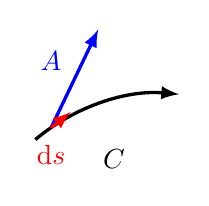
\begin{tikzpicture}
\draw [-latex,very thick](-1,0)  arc [start angle=130,delta angle=-45,radius=2.5] ; 
\node [below] {$C$} ; 
\draw [-latex,very thick,draw=blue] (-0.8,0.15) -- (-0.2,1.4) ;
\node at (-0.8,1) {\textcolor{blue}{$\bm{A}$}} ; 
\draw [-latex,very thick,draw=red] (-0.8,0.15) -- (-0.55,0.35) ; 
\node at (-0.8,-0.2) {\textcolor{red}{$\mathrm{d} \bm{s}$}} ; 
\end{tikzpicture}
\end{center}

$C$の各地点における$\mathrm{d}\bm{s}$と
その場所での$\bm{A}(\bm{r})$との内積$\bm{A}(\bm{r}) \cdot \mathrm{d}\bm{s}$をとる. 
$\mathrm{d}\bm{s}$は$C$のどの地点を考えるかで違うベクトルになることに注意しておこう. 
試しに3ヶ所くらい図に書いてみるといいだろう. 

そして, その内積の値を$C$上全体にわたって足し合わせる. 無限個の実数の足し算である. これを
\begin{eqnarray}
\int_{C}^{} \bm{A}(\bm{r}) \cdot \mathrm{d} \bm{s} 
\label{eq:sensekibun}
\end{eqnarray}
と書き,この積分を
\textbf{\textcolor{red}{ベクトル場$\bm{A}(\bm{r})$の曲線$C$上における線積分}}\index{せんせきふん@線積分}と定義するのである. 

内積$\bm{A}(\bm{r}) \cdot \mathrm{d} \bm{s}$というのは$\bm{A}(\bm{r})$の$\mathrm{d} \bm{r}$方向の
長さを表しているのだった. また, $\mathrm{d}\bm{s}$は$C$と同じ向きである. 
すなわち, ベクトル場の線積分は\textbf{\textcolor{red}{ベクトル場がその曲線状にどれだけ沿って分布しているかを表していることになる.}}
曲線とほぼ同じ方向にベクトル場が分布していれば線積分の値は大きくなるし, 
ベクトル場が曲線とずっと垂直であれば線積分の値は0になる. 
線積分とはそういうものである. 具体的に線積分を計算したければ曲線をパラメーター表示するのが手っ取り早いだろう. 
そういう問題は普通の教科書であれば必ず載っていることだろうから本書では省略させてもらおう. 

\subsubsection{閉曲線での線積分はベクトル場の回転を表す}
ベクトル場の線積分が真価を発揮するのは曲線が閉曲線である場合である. 
ベクトル場を閉曲線上で線積分すると, その値はベクトル場がどれだけ強い渦を巻いているかを表しているのである. 
このことについて少し考えてみよう. 

閉曲線$C_0$というものを考える. 閉曲線というのは始点と終点が一致しているような直線である. 
何かしらの経路が「閉じている」ときに, その経路を表す記号の下に0を付けて「これは閉じた経路ですよ」
ということを表すことがある. 閉曲線であれば曲線を表す記号$C$に下付き文字で0を付けて$C_0$と表すし, 
閉曲面であれば曲面を表す記号$S$に0を付けて$S_0$と表すという感じである. 

閉曲線に沿ってベクトル場を線積分するとき, それは始点から始まってぐるっと一周して戻ってくるイメージである. 
このイメージを強調するために, $\int$記号に丸をくっつけて
\begin{eqnarray}
\oint_{C_0}^{} \bm{A}(\bm{r}) \cdot \mathrm{d} \bm{s} 
\label{eq:sensekibunhei}
\end{eqnarray}
と書き表すことがある. この積分は\textbf{\textcolor{red}{周回積分}}\index{しゆうかいせきふん@周回積分}と呼ばれるものである. 
ただし, 周回積分であっても積分記号に丸をつけないことも多いので, 丸をつけるかどうかは好みでよい. 
本書では周回積分は丸をつけた式(\ref{eq:sensekibunhei})のような形で表すことにする. 

ベクトル場の閉曲線における線積分は何を表すだろうか? 
線積分はベクトル場が積分領域である曲線状に沿った分布を抽出するものであった. 
いま, その曲線は閉曲線である. ぐるっと一周回って戻ってくるイメージである. 
つまり, このベクトル場の閉曲線における線積分はベクトル場のぐるっと一周回ってもどってくるような
分布がどのくらいあるかを抽出するものなのである. 
わかりやすく言い換えよう. 
\textbf{\textcolor{red}{ベクトル場の閉曲線における線積分は, そのベクトル場がどのくらいの強さの渦を巻いているかを表している.}}
ぐるぐる渦を巻いているようなベクトル場の周回積分の値は大きくなるし(回転の向きによって正負があるが), 
まったく渦を巻いていないようなベクトル場の周回積分の値は0になる. 
この「渦なしの場」に関してはもう少し掘り下げてみよう. 

\subsubsection{渦なし場とスカラーポテンシャル}
まったく渦が存在しないようなベクトル場を考えてみよう. 
これは, 式(\ref{eq:sensekibunhei})が
\textbf{\textcolor{red}{任意の}}\footnote{「任意」と「存在」の意味の違いくらいはわかるよな?} 閉曲線$C_0$について
成り立つようなベクトル場について考えるという意味である. 
このような場は\textbf{\textcolor{red}{渦なしの場}}\index{うすなしのは@渦なしの場}と呼ばれている. 

さて, 渦なしの場$\bm{A}(\bm{r})$については次のような式が成り立っているのだった. 
\begin{eqnarray}
\oint_{C_0}^{} \bm{A}(\bm{r}) \cdot \mathrm{d} \bm{s} = 0
\label{eq:uzunasi}
\end{eqnarray}
ある点から別の点に至る経路のうち, 始点と終点が同じで途中経過が異なる曲線$C_1$, $C_2$について考える. 
$C_2$の終点からスタートして$C_2$に沿ってその始点に向かうような経路を$-C_1$と表す. 
$-C_2$という経路はちょうど曲線$C_2$を真逆の向きに走るコースである. 図を描いてみればすぐにわかるだろう. 
始点から経路$C_1$に沿って終点に向かい, その終点から今度は経路$-C_1$に沿って始点に戻ってくる経路を考える. 
この経路は$C_1$と$-C_2$の合成である. この経路を$C_1+(-C_2)$と表すことが多い. 
これをさらに略記して$C_1-C_2$と書く. 経路$C_1-C_2$は閉曲線である. 
したがって式(\ref{eq:uzunasi})が成り立つ. 
$$
\oint_{C_1-C_2}^{} \bm{A}(\bm{r}) \cdot \mathrm{d} \bm{s} = 0
$$
さて, 
$$
\oint_{C_1-C_2}^{} \bm{A}(\bm{r}) \cdot \mathrm{d} \bm{s} = 
\int_{C_1}^{} \bm{A}(\bm{r}) \cdot \mathrm{d} \bm{s} + \int_{-C_2}^{} \bm{A}(\bm{r}) \cdot \mathrm{d} \bm{s}
$$
が成り立つし, 
$$
\int_{-C_2}^{} \bm{A}(\bm{r}) \cdot \mathrm{d} \bm{s} = 
- \int_{C_2}^{} \bm{A}(\bm{r}) \cdot \mathrm{d} \bm{s}
$$
が成り立っている. 意味を考えれば明らかである. これは各自確認しておいてもらいたい. 

これにより, 
\begin{eqnarray*}
\int_{C_1}^{} \bm{A}(\bm{r}) \cdot \mathrm{d} \bm{s} - \int_{C_2}^{} \bm{A}(\bm{r}) \cdot \mathrm{d} \bm{s} = 0 \\
\therefore \; \; 
\int_{C_1}^{} \bm{A}(\bm{r}) \cdot \mathrm{d} \bm{s} = \int_{C_2}^{} \bm{A}(\bm{r}) \cdot \mathrm{d} \bm{s}
\end{eqnarray*}
が成り立つことになる. $C_1$と$C_2$は始点と終点が一致するように任意にとったのであった. この式から言えるのは, 
\textbf{\textcolor{red}{渦なしの場における線積分の値は途中経路に依存せず, 始点と終点のみで決まる}}ということである. 
というわけで, 渦なしの場$\bm{A}(\bm{r})$について, 次のような式で定義されるスカラー$\phi(\bm{r})$を考える. 
\begin{eqnarray}
\phi (\bm{r}) = \int_{\bm{r}_0}^{\bm{r}} \bm{A}(\bm{r}) \cdot \mathrm{d} \bm{s}
\label{eq:sukara}
\end{eqnarray}
$\bm{r}_0$というのはどこかに適当にとった基準点である. 別にどこでもいい. $\bm{r}_0$がどこだろうと大した問題ではない. 
積分範囲を$\bm{r}_0$から$\bm{r}$としてあるが, これは$\bm{r}_0$を始点, $\bm{r}$を終点とする適当な曲線をとり, 
その曲線上で$\bm{A}(\bm{r})$を線積分してくれという意味である. 
どの曲線をとるかで$\phi(\bm{r})$の値が変わらないことはさっき確認したとおりである. 
$\phi(\bm{r})$は$\bm{r}$によって値がきまる1つのスカラーである. 
$\phi(\bm{r})$を$\bm{A}(\bm{r})$の
\textbf{\textcolor{red}{スカラーポテンシャル}}\index{すからーぽてんしやる@スカラーポテンシャル}という. 

スカラーポテンシャルに関して深堀りするのはやめておこう. 
とにかく, 渦なしの場に対しては経路によらない線積分としてスカラーポテンシャルが定義できるのである. 
渦のある場に対してはこのようなことは言えない. 線積分に値が経路によって変化してしまうためである. 
このような場合にはスカラーポテンシャルに加えてベクトルポテンシャルなるものを使う. 
経路によって線積分の値が変わるのが問題なのであれば, 
ポテンシャルに向きを付加すればどうにかなるんじゃね? くらいのノリである. 
Maxwell方程式にたどり着くまでの電磁気学を学ぶくらいでは, ベクトルポテンシャルはとりあえず必要になることもないだろう. 

\begin{itembox}[l]{課題}
ベクトル場$\bm{E}(\bm{r})$が
$$
\bm{E}(\bm{r}) = \frac{1}{4 \pi \varepsilon_0} \frac{q}{r^2} \frac{\bm{r}}{r}
$$
と与えられたとき, \textbf{\textcolor{red}{任意の}}閉曲線$C_0$について
\begin{eqnarray}
\oint_{C_0} \bm{E}(\bm{r}) \cdot \mathrm{d}\bm{s} = 0
\label{eq:Euzunasi}
\end{eqnarray}
が成り立っていることを確かめよ. 式(\ref{eq:Euzunasi})は静電場が渦なし場であることを示している. 
極座標系において, $r$, $\theta$, $\phi$がそれぞれ$\mathrm{d}r$, $\mathrm{d}\theta$, $\mathrm{d}\phi$
だけ変化したとき, $\mathrm{d}\bm{s}$が
$$
\mathrm{d}\bm{s} = \left[
\renewcommand{\arraystretch}{1}
\begin{array}{c}
\mathrm{d}r \\
r \, \mathrm{d}\theta \\
r \sin \theta \, \mathrm{d} \phi
\end{array}
\right]
$$
と表せることにさえ納得できればあとは簡単である. 
\end{itembox}
\subsubsection{ベクトル場の面積分}
線積分がベクトル場を線上で積分するのなら, 面積分はベクトル場を面上で積分する手法である. 
やることはさっきと変わらない. まず積分領域を無限に細かく分割して, 
その各地点で微小量を作り, 最後にその総和をとる. 思えば積分というのはみんなそんなものだった. 

ベクトル場$\bm{A}(\bm{r})$と空間上の曲面$S$を考える. 
積分する都合上, 曲面$S$には表と裏があるということにしておこう. 
表と裏が明確に区別することができない曲面というものはあるものの, そういうものは考えないことにする. 
まず, $S$を非常に細かい微小面に分割する. 分割された各微小面の面積は$\mathrm{d}S$であるとしておこう. 
そして, 分割された各微小領域上にその面に垂直で, 向きは面の表側を向いていて, 
かつ大きさが1であるようなベクトル$\bm{n}$をとる. $S$は曲面であるから, 垂直といっても
どの向きを向いたらいいのかわからない. しかし, 微小面に分割してしまえばそれはもはや平面といっても差し支えない. 
平面であればそこに垂直なベクトルを考えることができるだろう. 
\begin{center}
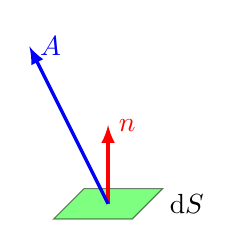
\begin{tikzpicture}
\filldraw [draw=black,fill=green,opacity=0.5] (1,0,1) -- (1,0,2) -- (2,0,2) -- (2,0,1) -- (1,0,1) ; 
\node at (2.5,0,1.5) {$\mathrm{d}S$} ; 
\draw [-latex,very thick,draw=red] (1.5,0,1.5) -- (1.5,1,1.5) node [right] {\textcolor{red}{$\bm{n}$}} ; 
\draw [-latex,very thick,draw=blue] (1.5,0,1.5) -- (0.5,2,1.5) node [right] {\textcolor{blue}{$\bm{A}$}} ; 
\end{tikzpicture}
\end{center}
$S$上の各面において, $\bm{A}(\bm{r})$と$\bm{n}$の内積をとり, その面の面積$\mathrm{d}S$をかけてやる. 
そして, この量を曲面$S$全体について総和をとる. この積分を
\begin{eqnarray}
\int_{S} \bm{A}(\bm{r}) \cdot \bm{n} \, \mathrm{d}S
\label{eq:mensekibun}
\end{eqnarray}
と書き, これをベクトル場$\bm{A}(\bm{r})$の曲面$S$における\textbf{\textcolor{red}{面積分}}\index{めんせきふん@面積分}
と定義するのである. 

流儀によっては$\bm{n}\, \mathrm{d}S$を$\mathrm{d}\bm{S}$と1つにまとめてしまい, ベクトル場の面積分を
\begin{eqnarray}
\int_{S} \bm{A}(\bm{r}) \cdot \mathrm{d}\bm{S}
\label{eq:mensekibun2}
\end{eqnarray}
と定義してしまう流儀もある. この$\mathrm{d}\bm{S}$は分割された微小面に垂直で, その面の表方向を向いており, 
かつ大きさが$\mathrm{d}S$であるようなベクトルである. 
$\mathrm{d}\bm{S}$は\textbf{\textcolor{red}{面積素ベクトル}}\index{めんせきそへくとる@面積素ベクトル}, 
もしくは\textbf{\textcolor{red}{面素ベクトル}}\index{めんそへくとる@面素ベクトル}と呼ばれている. 

また, 面積分は2次元の積分領域での積分である. というわけで, 面積分を$\int$記号を2つ書いて
\begin{eqnarray}
\iint \bm{A}(\bm{r}) \cdot \bm{n} \, \mathrm{d}S
\end{eqnarray}
と表すような流儀もある. 
本書では式(\ref{eq:mensekibun})を主に使うことにする. 

\subsubsection{面積分は何を表すか}
面積分が何を表しているか考えてみよう. 
面積分の定義式(\ref{eq:mensekibun})を眺めてみると, $\bm{A}(\bm{r})$と$\bm{n}$の内積が入っている. 
これが表すのは$\bm{A}(\bm{r})$が$\bm{n}$方向にどれだけの成分を持っているかである. 
$\bm{n}$は$S$と垂直なのだった. 
つまり, $\bm{A}(\bm{r}) \cdot \bm{n}$は$\bm{A}(\bm{r})$の$S$に垂直な方向の成分を表していることになる. 
これにその面の面積$\mathrm{d}S$をかければ, 
それは$\bm{A}(\bm{r})$の$S$に垂直な方向の成分が$\mathrm{d}S$分だけありますよという意味になる. 
面積分は, この量を曲面$S$全体にわたって総和をとるのだ. 
すなわち, 面積分は\textbf{\textcolor{red}{ベクトル場$\bm{A}(\bm{r})$が曲面$S$の裏から表に垂直に貫くような
分布がどれだけあるかということを表している.}}
水の流れをイメージしてもらえるとわかりやすい. 
川があって, 場所を指定するとその場所での川の流れの方向と勢いをベクトルで返すような対応関係を考えれば, これはベクトル場となる. 
ここに面を適当にとり, その面で面積分してやる. 川の流れが強ければ強いほどこの面積分の値は大きくなるが, 
川が面に対して垂直に流れていなければ, その分値は小さくなる. 
面の表から裏に川が流れていれば, 面積分の値は負になる. 式(\ref{eq:mensekibun})でいえば, 
$\bm{A}(\bm{r})$と$\bm{n}$の向きが逆になるため, 内積の値が負になるのである. 

\subsubsection{重要なのはやっぱり閉曲面}
面積分で特に重要なのは閉曲面に関する面積分である. 閉曲面というのはざっといえば球面のようなイメージである. 
閉曲面の外側が表側で, 内部が裏側である. 
閉曲面上での面積分は次のように表す. 
\begin{eqnarray}
\oint_{S_0} \bm{A}(\bm{r}) \cdot \bm{n} \, \mathrm{d}S
\label{eq:heimensekibun}
\end{eqnarray}
積分領域が「閉じている」ことを表すのに$S$の下に0をつけて$S_0$と表すし, $\int$記号を$\oint$に変更してあるのである. 
これは線積分のときと同じ書き方である. 

\subsubsection{閉曲面上での面積分はベクトル場の発散を表す}
ベクトル場を閉曲面上で面積分したとき, 
その値はベクトル場がその閉曲面からどれだけ発散しているかを表す. 
これについて考えてみよう. 

まず, 面積分はその面の裏から表へ垂直に貫く場の分布を表すのだった. 
今は積分領域を閉曲面としている. 閉曲面の裏側というのは曲面の内側で, 表側というのは曲面の外側のことであった. 
裏から表へ垂直に貫く場の分布というのは, まさに曲面の内側から外側へ貫く場の分布である. 
これはつまりベクトル場の湧き出し, すなわち発散に他ならない. 
すなわち, \textbf{\textcolor{red}{ベクトル場の閉曲面上での面積分は, そのベクトル場の
曲面内部からの発散を表す}}のである. 
なお, 面積分の値が負になるのは外側から内側へ貫く場の分布があるときであるから, 
このときには面積分の値はベクトル場の吸い込みを表していることになる. 
値の正負の違いしかないので, 湧き出しも吸い込みもひとくくりにしてしまって「発散」と言っている. 
同じ式で表せる量なのだから言葉は1つの方がよかろ? 

さて, 曲面に沿ってぐるぐる回るような分布をしているようなベクトル場があったとき, 
そのベクトル場の発散は0になるべきである. 
実際, 式(\ref{eq:heimensekibun})にしたがって計算しても値は0になっている. 
これは, 各場所での内積がすべて0になるのからである. 直交している2つのベクトルの内積は0になるのだった. 
曲面に沿ってぐるぐる回っているような分布をしているベクトル場を考えるとき, 
あらゆる場所においてそのベクトルは面素ベクトルと直交している. 
和をとる前から値が0になっているのである. わざわざ$\bm{n}$などというベクトルを用意して内積をとった恩恵の1つである. 

ただし, ベクトル場の発散が0になるのはこのような場合だけではない. たとえどこかで局所的にベクトル場が発散していたとしても, 
別の場所で同じくらいのベクトル場の吸い込みが存在していれば, 積分したときに打ち消しあって総和としては0になる. 
これはベクトル場が曲面内部に入った分だけ出て行った, もしくは出て行った分だけ入ったということを意味しているのだから, 
発散が0になるのも納得である. 

以上がベクトル場の線積分と面積分の大雑把な説明である. 
イメージがついていれば, そのイメージはこういうものをがっつり数学的に勉強するときに大きな助けになる. 
それを実感してもらうために1つ演習をしよう. 
\begin{itembox}[l]{課題}
「立体角」という用語について調べ, ベクトル場$\bm{E}(\bm{r})$が
$$
\bm{E}(\bm{r}) = \frac{1}{4 \pi \varepsilon_0} \frac{q}{r^2} \frac{\bm{r}}{r}
$$
と与えられたとき, \textbf{\textcolor{red}{任意の}}閉曲面$S_0$について
\begin{eqnarray}
\oint_{S_0} \bm{E}(\bm{r}) \cdot \bm{n} \, \mathrm{d}S = \frac{q}{\varepsilon_0}
\label{eq:Egauss}
\end{eqnarray}
が成り立っていることを確かめよ. 
式(\ref{eq:Egauss})はまさに電場に関する\ruby{Gauss}{ガウス}の法則である. ぜひチャレンジしてもらいたい. 
\end{itembox} 
\section{微分演算子$\nabla$について}
電磁気学を学んでいるとよくこんなのが出てくる. 
\begin{eqnarray}
\nabla = \left[
 \begin{array}{c}
\displaystyle
\frac{\partial}{\partial x} \\
\displaystyle
\frac{\partial}{\partial y} \\
\displaystyle
\frac{\partial}{\partial z} 
 \end{array}
\right]
\label{eq:nabla}
\end{eqnarray}
この記号$\nabla$は\textbf{\textcolor{red}{ナブラ}}\index{なふら@$\nabla$(ナブラ)}と読む. 
$\nabla$はベクトル(っぽいもの)である. よって手書きでは線を一本追加して二重文字で書く. 
$\nabla$は\textbf{\textcolor{red}{微分演算子}}の一種であるとよく言われる. 
$\nabla$は初学者キラーといっても過言ではないだろう. 多くの人がこいつに苦しめられてきたにちがいない. 
かくいう私もその1人である. だが, $\nabla$というのは単体ではまったく意味をなさない. 
この記号を用いることで多くの式が簡便に, かつ統一的に表現できて便利だから使っているにすぎないのだ. 
初学者の多くは$\nabla$単体の意味を必死に考え, そして挫折する. 
だが, 意味をもつのは$\nabla$単体ではなくそれを使って構成される種々の量である. 
それを今から考えてみよう. 
\subsubsection{微分演算子とは何か}
$\nabla$について考える前に, 「演算子」, そして「微分演算子」というものについて考えてみよう. 

それ単体では機能せず, 他のものに対して何かしらの計算の指示を与えるものを
\textbf{\textcolor{red}{演算子}}という. 数学者はよく「作用素」と呼んでいる. 
「計算の指示」というと堅苦しく聞こえるかもしれないが, $\sin$とか$\ln$とか, 
そんな感じのものが演算子である. 
$\sin$や$\ln$というのは後ろのモノに対して
その正弦の値や自然対数\footnote{自然対数というのは底が
Napire数$e$であるような対数のこと. 数学では普通$\log$という記号で表すが, 
物理をはじめとした自然科学では$\ln$と表すことが多い. 記号法のギャップに気をつけよ.} の値を計算してくれ, という記号である. 
和を表す記号$+$や積を表す記号$\times$も演算子の一種である. 
また, 演算子の中で後ろの関数を微分してくれ, という指示を含むような演算子のことを
\textbf{\textcolor{red}{微分演算子}}という. $\displaystyle \frac{\mathrm{d}}{\mathrm{d}x}$
や$\displaystyle \frac{\partial}{\partial x}$などは微分演算子である. 

さらに, 何かしらのモノに演算子をくっつけて実際に計算をさせることを演算子を\textbf{\textcolor{red}{作用させる}}という. 
なんだか偉そうに聞こえるが, 大した言葉ではない. 日常的にやっていることである. 
例えば, 数$x$の自然対数をとるという操作は「$x$に対して演算子$\ln$を作用させる」と言い換えることができるし, 
$x$, $y$関数$f(x, \, y)$を$x$で偏微分するという操作は「関数$f$に微分演算子$\displaystyle \frac{\partial}{\partial x}$を作用させる」
と言い換えることができる. 言葉を言い換えるだけでなんだかとても高尚なことをやっている気分になる. 
演算子というものに対してはそのくらいの気持ちで付き合っていけばいいのだ.  

演算子というものを考えると式を略記できることがある. 例えば, 
$$
\frac{\partial^2 f}{\partial x^2} + \frac{\partial^2 f}{\partial y^2} + \frac{\partial^2 f}{\partial z^2}
$$
という式があったときに, これは
$$
\left( \frac{\partial^2}{\partial x^2} + \frac{\partial^2}{\partial y^2} + \frac{\partial^2}{\partial z^2} \right) f
$$
と略記できる. この記法は式を簡潔に記述するだけでなく, 式に隠れた対称性や規則性を浮き彫りにしてくれることがある. 

\subsubsection{演算子は順番に気を付けろ}
使うのにはとっても便利な演算子であるが, \textbf{\textcolor{red}{演算子は作用させる順番によって結果が変わることがある.}}
このことに気を付けないまま計算を進めた結果, なんだかよくわからないものが得られてしまったりするので気を付けなければならない. 

例として微分演算子でやってみよう. 微分演算子$\displaystyle \frac{\mathrm{d}}{\mathrm{d}x}$と
演算子としての関数$g$があったとする. 関数$f$に$g$を作用させる, というのはその積$gf$をとれ
という計算をさせることだと解釈しておく. 

まず, 関数$f$に$\displaystyle \frac{\mathrm{d}}{\mathrm{d}x}$を作用させてから$g$を作用させてみる. 
結果は
$$
g \left( \frac{\mathrm{d}f}{\mathrm{d}x} \right)  = g \frac{\mathrm{d}f}{\mathrm{d}x}
$$
となる. 特に変わったところはない. 

次に, $g$を作用させてから$\displaystyle \frac{\mathrm{d}}{\mathrm{d}x}$を作用させてみよう. 
結果は
$$
\frac{\mathrm{d}}{\mathrm{d}x} (gf) = f \frac{\mathrm{d}g}{\mathrm{d}x} + g \frac{\mathrm{d}f}{\mathrm{d}x}
$$
となり, 前者とは違った結果になってしまう. 
演算子に関しては交換法則は成り立っていないのである. 
座標変換などを考えるときにそういうことに出くわすことがあるだろう. 
そのときになったら気を付けてもらえばいい. 

\subsubsection{$\nabla$を使ってみよう}
演算子というのはそれ単体では大した意味を持たないことが多いというのはわかってもらえただろうか. 
$\nabla$もそうである. $\nabla$単体の意味をどう解釈してみようか努力してみてもまったくの無駄である. 
それよりも, $\nabla$を使って構成される量の方に興味があるのである. 
本書ではスカラー場の勾配を表すグラーディエント, ベクトル場の発散を表すダイバージェンス, 
そしてベクトル場の回転を表すローテーション(もしくはカール)の3つを学ぶ. 

\subsubsection{ベクトル場の勾配}
スカラー場$\phi(x, \, y, \, z)$があったとする. これに$\nabla$を作用させてベクトルを作ってみよう. 
\begin{eqnarray}
\nabla \phi = \left[
 \begin{array}{c}
\displaystyle
\frac{\partial \phi}{\partial x} \\
\displaystyle
\frac{\partial \phi}{\partial y} \\
\displaystyle
\frac{\partial \phi}{\partial z} 
 \end{array}
\right]
\label{eq:gradnabla}
\end{eqnarray}
というベクトルができた. このベクトルをスカラー場$\phi$の\textbf{\textcolor{red}{勾配}}という. 
このベクトルは, 各点$(x, \, y, \, z)$に対し, $\phi$が最も急激に増加するような方向を指し示している. 
そういうわけで「勾配」などといういかつい名前がついているのである. 
と言われても, この式を見せられただけで納得できるような人はまずいない. 
しかし, ちょっと考えればすぐにわかるのである. 

$\phi$の全微分は
$$
\mathrm{d} \phi = \frac{\partial \phi}{\partial x} \mathrm{d} x 
+ \frac{\partial \phi}{\partial y} \mathrm{d} y +  \frac{\partial \phi}{\partial z} \mathrm{d} z
$$
であった. よく見ると, $\phi$の全微分$\mathrm{d}\phi$は位置の微小変化$\mathrm{d}\bm{r}$と
$\phi$の勾配$\nabla \phi$の内積になっているではないか. 
つまり, $\phi$の微小変化$\mathrm{d}\phi$は位置の微小変化$\mathrm{d}\bm{r}$が
$\nabla \phi$の方向を向いているときに最も大きくなるのである. 
こうしてみると, 「勾配」というネーミングにも納得である. 

また, 「勾配」は英語でgradientと表す. そういうわけで, スカラー場の勾配を
\begin{eqnarray}
\mathrm{grad} \, \phi = \left[
 \begin{array}{c}
\displaystyle
\frac{\partial \phi}{\partial x} \\
\displaystyle
\frac{\partial \phi}{\partial y} \\
\displaystyle
\frac{\partial \phi}{\partial z} 
 \end{array}
\right]
\label{eq:gradgrad}
\end{eqnarray}
というように表す流儀もある. 好きな方を使えばいいが, どちらの記号が出てきても混乱しないようにはしておくべきだ. 
本書では, 式(\ref{eq:gradgrad})を主に用いる. 
\subsubsection{ベクトル場の発散}
$\nabla$はベクトルっぽいものであった. であれば, ベクトル場$\bm{A}(\bm{r})$について, 
$\bm{A}(\bm{r})$と$\nabla$の内積を考えることができるだろう. そしてそれは
\begin{eqnarray}
\nabla \cdot \bm{A} (\bm{r}) =  \frac{\partial A_x}{\partial x} + \frac{\partial A_y}{\partial y} +  \frac{\partial A_z}{\partial z}
\label{eq:divnabla}
\end{eqnarray}
と書き表されるだろう. ベクトル場から1つのスカラーを得た. 
これをベクトル場$\bm{A}(\bm{r})$の\textbf{\textcolor{red}{発散}}という. 
この量は各点$(x, \, y, \, z)$に対し, その地点からベクトル場$\bm{A}(\bm{r})$がどれだけ湧き出しているかを表している. 
そういうわけでこの量は発散と呼ばれているのである. 全微分と似ているが, ちょっと違う. 
微分されているのは$\bm{A}(\bm{r})$自身ではなく, その各成分である. 

$x$, $y$, $z$のうち$x$だけが微小量$\mathrm{d}x$だけ変化したとき, $A_x$の微分$\mathrm{d} A_x$は
$$
\mathrm{d} A_x = \frac{\partial A_x}{\partial x} \mathrm{d}x
$$
と表されるのだった. 
同様にして, $y$だけが微小量$\mathrm{d}y$だけ変化したとき, $A_y$の微分$\mathrm{d} A_y$は
$$
\mathrm{d} A_y = \frac{\partial A_y}{\partial y} \mathrm{d}y
$$
と表されるし, $z$だけが微小量$\mathrm{d}z$だけ変化したとき, $A_z$の微分$\mathrm{d} A_z$は
$$
\mathrm{d} A_z = \frac{\partial A_z}{\partial z} \mathrm{d}z
$$
と表される. この式に対して疑問がわくようであれば, 再度偏微分のところの解説か, 常微分の解説に戻っていただきたい. 

もし$x$が増加して$A_x$が増加すれば, 
それはその場所からベクトル場の$x$成分が湧いて出てきたと考えるほかはない. 
「$x$が増加した」を「ある点よりも$x$軸方向に進んだ点を見た」と言い換えてみるとわかりやすいかもしれない. 
ほかの成分に関しても同様である. $x$が変化したときに$\bm{A}(\bm{r})$の$y$成分や$z$成分の変化を考えないのは, 
たとえ$y$成分や$z$成分が変化したとしても, 
それはベクトル場の$y$成分や$z$成分が湧いて出てきたと考えることはできないからである. 
各自図を描いて確認してほしい. こういうことには大いに悩むべきである. 

式(\ref{eq:divnabla})は各軸方向の発散の総和である. 
たとえ$x$軸の方向にベクトル場が湧き出していたとしても, 
同じくらい$y$軸方向にベクトル場の吸い込みが発生していたとするならば, 
それはベクトル場の発散があるというべきではないだろう. 和をとっているのはそういう意味である. 

「発散」は英語でdivergenceという. そんなわけで, ベクトル場の発散を$\nabla$を使わずに
\begin{eqnarray}
\mathrm{div} \, \bm{A}(\bm{r}) = \frac{\partial A_x}{\partial x} + \frac{\partial A_y}{\partial y} +  \frac{\partial A_z}{\partial z}
\label{eq:divdiv}
\end{eqnarray}
と表記することもある. これも好きな方を使うといい. 
どちらの書き方が使われていてもきちんと読めるようにしておこう. 
本書では, 主に式(\ref{eq:divdiv})を用いることにする. 
\subsubsection{\ruby{Gauss}{ガウス}の定理}
さて, $\mathrm{div} \, \bm{A}(\bm{r})$は各点$(x, \, y, \, z)$におけるベクトル場の発散を表しているのだった. 
ところが, ベクトル場の発散といえば閉曲面上でベクトル場を面積分することでも得られたはずだ. 

閉曲面上でベクトル場を面積分することで得られたのは, その閉曲面の内側から外側へのベクトル場の発散の合計であった. 
一方, $\mathrm{div}\bm{A}(\bm{r})$が表すのは各点$(x, \, y, \, z)$での発散である. 
これを閉曲面$S_0$の内部全体にわたって足し合わせれば, $S_0$の内側から外側への発散の合計が得られるはずだ. 
積分領域は3次元領域であるから, これを$V$と表記しておこう. 
この積分は, $V$を細かいさいころのようなブロックに分割して足し合わせていくイメージである.  
すると, 次のような等式が成り立っているはずだ. 
\begin{eqnarray}
\int_V \mathrm{div} \, \bm{A}(\bm{r}) \, \mathrm{d}V = \oint_{S_0} \bm{A}(\bm{r}) \cdot \bm{n} \, \mathrm{d}S
\label{eq:Gaussthe}
\end{eqnarray}
ただし, $V$は$S_0$内部全体である. 式(\ref{eq:Gaussthe})を
\textbf{\textcolor{red}{\ruby{Gauss}{ガウス}の定理}}\index{かうすのていり@Gaussの定理}と呼ぶ. 
詳しい導出はやらない. その代わり式の解釈をしておこう. 式(\ref{eq:Gaussthe})の両辺をよく眺めてほしい. 
左辺の積分領域は$V$, つまり3次元領域で, 右辺の積分領域は$S_0$, つまり2次元領域である. 
\ruby{Gauss}{ガウス}の定理を利用するときにはこの性質をうまく利用することが多い. 
つまり, \ruby{Gauss}{ガウス}の定理は積分領域を変更したいときに使われるのである. 
たとえば, \ruby{Maxwell}{マクスウェル}方程式を微分形から積分形, もしくはその逆に変形するときにこの定理は使われる. 

とはいえ, いま理解すべきは左辺と右辺がともにベクトル場の発散を表しているということだ. 
それさえ納得できてしまえば式(\ref{eq:Gaussthe})を忘れることもないだろう. 
\subsubsection{ベクトル場の回転}
さっきやったのは$\nabla$とベクトルの内積である. 今度は$\nabla$とベクトルの外積を考えてみよう. 
何も考えずに計算してみれば, このようなベクトルが得られるはずだ. 
\begin{eqnarray}
\nabla \times \bm{A}(\bm{r}) = \left[
\begin{array}{c}
\displaystyle
\frac{\partial A_z}{\partial y} - \frac{\partial A_y}{\partial z} \\
\displaystyle
\frac{\partial A_x}{\partial z} - \frac{\partial A_z}{\partial x} \\
\displaystyle
\frac{\partial A_y}{\partial x} - \frac{\partial A_x}{\partial y} 
\end{array}
\right]
\label{eq:rotnabla}
\end{eqnarray}
ベクトルの外積の成分表示のところをじっくり見ながら計算してみてほしい. 
ベクトル場からまた違うベクトルを得た. これをベクトル場$\bm{A}(\bm{r})$の
\textbf{\textcolor{red}{回転}}という. このベクトルは各点$(x, \, y, \, z)$に対し, 
その地点でベクトル場$\bm{A}(\bm{r})$がどの方向にどれだけの渦を巻いているかを表すベクトルである. 
このベクトルが「回転」と呼ばれているのはそこからきている. 
回転といってもいろいろな方向が考えられるだろう. 
ベクトル場の回転がまたベクトルになっているのはそういうことである. 
ベクトル場がどの向きに渦を巻いているかをしているかをその向きで, 
渦がどの程度の強さなのかをそのノルムによって表しているのである. 

いま何を言っているかよくわからない人は, おそらく力学で回転関係の話を
学んでいないか, もしくはきちんと数学的に定式化された形で学んでいないかのどちらかだろう. 
そういう人は多いだろうから, ざっくりとだが復習しておこう. 
\subsubsection{回転を1本のベクトルで表す}
1本ベクトルが持っている方向というのは1つである. これはまったく当たり前のことである. 
これだけで「回転」を表現するのは不可能に見えるかもしれない. 
川の流れがぐるぐると渦を巻いている様子を想像してみると, それぞれの点では流れの向きはばらばらである. 
しかし, 全体を見てみるとなんとなく渦を巻いている. そんなイメージである. 
この川の渦をたった1本のベクトルで表したい. 
それにはどうすればよいだろうか? 必要なのは回転軸という考え方である. 

ベクトルの外積のところで「2つのベクトル$\bm{a}$, $\bm{b}$について, 
その外積$\bm{a} \times \bm{b}$の向きは, $\bm{a}$から$\bm{b}$の向きに右ネジを回したとき, 
そのネジが進む方向であると定義する」と説明したのを覚えているだろうか. 
あの場面では先にネジが回転する方向がわかり, それをもとに外積の向きが決まったのであった. 
そう, 回転の向きとベクトルの向きが対応しているのである. 

「逆に考えることはできないだろうか? ベクトルの向きが回転の方向を決めていると考えるのである. 
それには「こういうベクトルにはこういう回転が対応しますよ」という約束事を指定しなくてはならない. 
どうせなら外積と同じにしてしまおう. 
\textbf{\textcolor{red}{あるベクトルが表す回転の向きは, そのベクトルの向きが右ネジが進む向きになるような
ネジの回転方向であると約束することにする.}}
回りくどい言い方だが, 要はベクトルの外積のときと同じ対応関係になるようにしたのである. 
ベクトルの大きさは, 回転の強さを表すことにしておこう. これは自然な考えである. 
大きさが大きいベクトルほどそのベクトルが表す回転は激しいのである. 

これで1本のベクトルと1つの回転が完全に対応付けられた. 
勘違いしてほしくないのだが, これはすべてのベクトルが回転を表すと決めたわけではない. 
もしこのベクトルが回転を表すとしたら, それはこういう回転方向と強さを表していますよ, 
というように約束事を作っただけである. 
力$\bm{F}$が回転を表しているわけなかろう? そんなニュアンスである. 

力学においてはこの約束事のもと, 回転に関する種々の物理量がベクトル化される. 
力のモーメント$\bm{N}$や角速度$\bm{\omega}$などである. 
このようにベクトルで表しておくと, いろいろな方向の回転に対して式を統一的に表現できて便利である. 
基準点からみて位置$\bm{r}$にある物体に力$\bm{F}$がはたらいているとき, 
その力のモーメントは$\bm{N}=\bm{r}\times\bm{F}$と書き表され, 
物体の角速度が$\bm{\omega}$であればその速度は$\bm{v}=\bm{\omega}\times\bm{r}$
と書き表される. 

もし外積の順序を逆にしてしまうと, ベクトルの向きと回転方向の対応関係が崩れてしまう. 
ベクトルの向きと回転方向の向きの対応関係は, 人間が式を読み解くときに使うもので, 
式そのものの中に回転方向が内蔵されているわけではないのである. 
たとえば角速度$\bm{\omega}$がいくら回転を表しているといっても, 
$\bm{\omega}$自体はただのベクトルである. 
これが約束した正しい方向の回転を表すように仕向けるためには, 
作った公式がうまく自身の方向と回転方向との関係を反映したものでなくてはならない. 
角速度$\bm{\omega}$の例でいえば, $\bm{v}=\bm{\omega}\times\bm{r}$という式がそれである. 

こうしてみると, 回転関係の式にベクトルの外積が頻繁に現れるのは必然であるといえるだろう. 
あれだけ難しく見えた外積も, 回転のベクトル表現も, 
1からきちんと考えてみれば, 決して難しい話ではないのだ. とはいえ,考えるべきことはまだある. 
\begin{itembox}[l]{検討}
いまの話では, 回転という現象をたった1本のベクトルで表せることを学んだ. 
「回転」と「渦」はほぼ同じ意味だと思ってもらって構わない. 

さて, 川に渦が巻いている状況を考えよう. 渦であるからそれはベクトルで表せるはずだ. 
しかし, 川の渦は場所によって強さが違う. 向きさえ一定ではないだろう. 

このような状況では, この川の渦をたった1本の定まったベクトルとして表すのは不可能である. 
いったいどうしたらいいだろう? 考えてみよ. 
\end{itembox}

\subsubsection{ベクトル場の回転について考える}
ちょっと(しかし重要な)脱線をしたところで, 話を戻そう. ベクトル場の回転というのは次の式で定義されるのだった. 
\begin{eqnarray}
\nabla \times \bm{A}(\bm{r}) = \left[
\begin{array}{c}
\displaystyle
\frac{\partial A_z}{\partial y} - \frac{\partial A_y}{\partial z} \\
\displaystyle
\frac{\partial A_x}{\partial z} - \frac{\partial A_z}{\partial x} \\
\displaystyle
\frac{\partial A_y}{\partial x} - \frac{\partial A_x}{\partial y} 
\end{array}
\right]
\label{eq:rotnabla2}
\end{eqnarray}
このベクトルがベクトル場$\bm{A}(\bm{r})$の回転を表しているというのであった. 
このことについて, 少し考えてみよう. とはいえ, 成分が3つあるので, まずは$z$成分から考えてみよう. 
なぜ$z$成分から考えるかというと, $\nabla \times \bm{A}(\bm{r})$の$z$成分が$\bm{A}(\bm{r})$の回転を表しているからである. 
このことは読めばすぐにわかるはずだ. とりあえず先に進もう. 

$\nabla \times \bm{A}(\bm{r})$の$z$成分は
\begin{eqnarray}
(\nabla \times \bm{A}(\bm{r}))_z = \frac{\partial A_y}{\partial x} - \frac{\partial A_x}{\partial y} 
\label{eq:rotnablaz}
\end{eqnarray}
である. ベクトルの成分を表すのに, そのベクトルに対応する成分を表す添え字をつけることがある. 
こういう表記は大概予告なしに使われることがあるので覚えておこう. 

さて, 式(\ref{eq:rotnablaz})が何を表しているのか考えてみよう. 
まずは第1項
$$
\frac{\partial A_y}{\partial x}
$$
からである. この項は$x$が変化したときの$\bm{A}(\bm{r})$の$y$成分の変化率を表しているのだった. 
もしこの項が正であれば, それは$x$軸の正方向に進めば進むほど$\bm{A}(\bm{r})$の$y$成分が増加していくことになる. 

第2項
$$
-\frac{\partial A_x}{\partial y}
$$
についても同じように考えてやる. この項は$y$が変化したときの$\bm{A}(\bm{r})$の$x$成分の変化率を表している. 
頭に$-$記号がくっついているので, 
この項が全体として正であるときには
$y$軸の正方向に進めば進むほど, $\bm{A}(\bm{r})$の$x$成分が減少していくことになる. 

すなわち, $x$に対して$\bm{A}(\bm{r})$の$y$成分が増加し, かつ$y$に対して$\bm{A}(\bm{r})$の$x$成分が減少するとき, 
$\nabla \times \bm{A}(\bm{r})$の$z$成分は正になっている. 
このような場合, $\bm{A}(r)$の分布はどうなっているだろうか? 図に書き起こしてみよう. 

\begin{center}
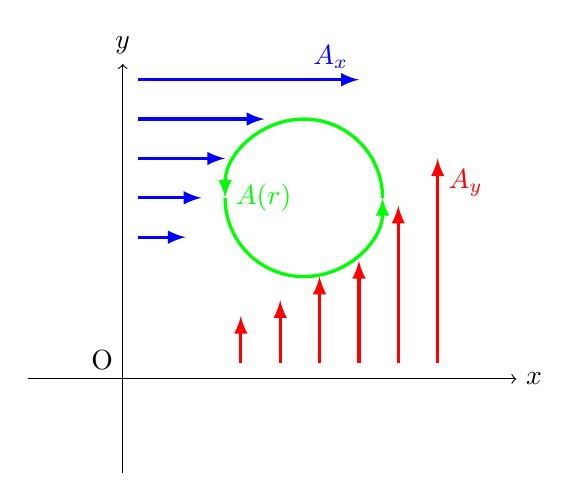
\begin{tikzpicture}[domain=-1:4] % グラフの描画領域は区間[-1, 4]
\draw[->] (-1.2,0) -- (5,0) node[right] {$x$} ; % x軸
\draw[->] (0.,-1.2) -- (0,4) node[above] {$y$} ; % y軸
\coordinate (0) at (0,0) ; 
\node [above left] (0) at (0,0) {$\mathrm{O}$}  ; % 原点
\draw [-latex,very thick,draw=red] (1.5,0.2) -- (1.5,0.8) ; 
\draw [-latex,very thick,draw=red] (2,0.2) -- (2,1) ;
\draw [-latex,very thick,draw=red] (2.5,0.2) -- (2.5,1.3) ; 
\draw [-latex,very thick,draw=red] (3,0.2) -- (3,1.5) ;
\draw [-latex,very thick,draw=red] (3.5,0.2) -- (3.5,2.2) ;
\draw [-latex,very thick,draw=red] (4,0.2) -- (4,2.8) 
node [below right] {\textcolor{red}{$A_y$}} ;
\draw [-latex,very thick,draw=blue] (0.2,3.8) -- (3,3.8) 
node [above left ] {\textcolor{blue}{$A_x$}} ;
\draw [-latex,very thick,draw=blue] (0.2,3.3) -- (1.8,3.3) ; 
\draw [-latex,very thick,draw=blue] (0.2,2.8) -- (1.3,2.8) ;
\draw [-latex,very thick,draw=blue] (0.2,2.3) -- (1,2.3) ; 
\draw [-latex,very thick,draw=blue] (0.2,1.8) -- (0.8,1.8) ; 
\draw [very thick,draw=green,-latex] (1.3,2.3) arc (180:360:1)  ;
\draw [very thick,draw=green,-latex] (3.3,2.3) arc (0:180:1) 
node [right] {\textcolor{green}{$\bm{A}(\bm{r})$}} ;
\end{tikzpicture}
\end{center}

\textcolor{red}{$A_y$}と\textcolor{blue}{$A_z$}の分布を見たときに, 
\textcolor{green}{$\bm{A}(\bm{r})$}の渦のようなものが見えていてほしい. 
$xy$平面を川だと思い, $\bm{A}(\bm{r})$を川の流れを表すベクトル場だと思ってみる. 
そして, この川の真ん中あたりに浮き輪を投げ込んだとき, 浮き輪がどう流れていくかを想像してもらえば納得がいくだろう. 

$xy$平面に時計回りの渦が発生しているとき, これを右ネジが回転する方向だと思うことにすると, 
右ネジは$z$軸正方向を進むことになる.(各自確かめよ)
したがって, この渦を表すベクトルは$z$軸正方向を向いているべきである. 
また, 図を見る限り, $A_y$と$A_x$の変化が激しいほど強い渦が発生していることになるだろう. 
これらのことから察するに, この渦を表しているのは$\nabla \times \bm{A}(\bm{r})$の$z$成分である. 
すなわち, $\nabla \times \bm{A}(\bm{r})$の$z$成分は
ベクトル場$\bm{A}(\bm{r})$の$xy$平面上にある渦の向きと強さを表しているのである. 

\begin{itembox}[l]{課題}
上の考察にならって, $\nabla \times \bm{A}(\bm{r})$の$x$成分や$y$成分が何を表しているかを調べよ.
\end{itembox}

$\nabla \times \bm{A}(\bm{r})$が$\bm{A}(\bm{r})$の回転を表していることにはもはや何の疑いもないだろう. 
そういうわけで, ベクトル場の回転を, 英単語rotationやcurlからとって
\begin{eqnarray}
\mathrm{rot} \, \bm{A}(\bm{r}) = \left[
\begin{array}{c}
\displaystyle
\frac{\partial A_z}{\partial y} - \frac{\partial A_y}{\partial z} \\
\displaystyle
\frac{\partial A_x}{\partial z} - \frac{\partial A_z}{\partial x} \\
\displaystyle
\frac{\partial A_y}{\partial x} - \frac{\partial A_x}{\partial y} 
\end{array}
\right]
\label{eq:rotrot}
\end{eqnarray}
だったり, 
\begin{eqnarray}
\mathrm{curl} \, \bm{A}(\bm{r}) = \left[
\begin{array}{c}
\displaystyle
\frac{\partial A_z}{\partial y} - \frac{\partial A_y}{\partial z} \\
\displaystyle
\frac{\partial A_x}{\partial z} - \frac{\partial A_z}{\partial x} \\
\displaystyle
\frac{\partial A_y}{\partial x} - \frac{\partial A_x}{\partial y} 
\end{array}
\right]
\label{eq:rotcurl}
\end{eqnarray}
というように表すことがある. rot表記は主に日本で, curl表記は主に海外で用いられることが多いようである. 
グローバルな読者の方々はcurl表記を主に使うのだろうか? 私は日本に引きこもりがちなのでrot表記がお気に入りである. 
好きなものを採用すればいいが, やはりどれが出てきても混乱しないようにはしておこう. 

\subsubsection{\ruby{Stokes}{ストークス}の定理}
$\mathrm{rot} \, \bm{A}(\bm{r})$はベクトル場$\bm{A}(\bm{r})$の回転を表すのだった. 
回転を表すといっても, $\mathrm{rot} \, \bm{A}(\bm{r})$はベクトル場で, 
$\bm{A}(\bm{r})$の各点$(x, \, y, \, z)$における局所的な回転を表している. 
これをある曲面$S$上全体にわたって面積分したらどうなるだろうか? ベクトル場の面積分が表しているのは
ベクトル場がその曲面を垂直に貫くような場の分布であった. 
いま積分するのは$\bm{A}(\bm{r})$自身ではなく$\mathrm{rot} \, \bm{A}(\bm{r})$である. 
$\mathrm{rot} \, \bm{A}(\bm{r})$が曲面を垂直に貫いているような分布がどれだけあるかを計算するということは, 
すなわちもとのベクトル場がその曲面にそってどのくらいの強さの渦を巻いているかを計算しているのと
同じことである.(本当だろうか? 考えてみよ)したがって, 曲面$S$のふちを$C_0$とすれば, $C_0$はもちろん閉曲線で
\begin{eqnarray}
\int_S \mathrm{rot} \, \bm{A}(\bm{r}) \cdot \bm{n} \, \mathrm{d} S =
\oint_{C_0} \bm{A}(\bm{r}) \cdot \mathrm{d}\bm{s}
\label{eq:Stokesthe}
\end{eqnarray}
という式が成り立っているということが推測できる. ただし, $S$は空間にある任意の曲面で, 
$C_0$はそのふちである. 
実際, 式(\ref{eq:Stokesthe})は厳密に成り立っていて, \textcolor{red}{\ruby{Stokes}{ストークス}の定理}と呼ばれている. 
\ruby{Gauss}{ガウス}の定理とよく似た形をした等式である. あちらと合わせて頭に叩き込んでしまおう. 

この式も\ruby{Gauss}{ガウス}の定理と同じく, 線積分を面積分に変換したり, またその逆を行ったりするときによく使われる. 
だが, とりあえず今確認すべきなのは, 
式(\ref{eq:Stokesthe})の両辺がともに$\bm{A}(\bm{r})$の回転を表しているということである. 


